\documentclass[./main.tex]{subfiles}
\begin{document}
\chapter{Grid Implementations for GORILLA}
\label{chap:GRID}
The developed code $GORILLA$ (Geometric ORbit Integration with Local Linearisation Approach) is a geometric guiding center orbit integrator written in \texttt{Fortran 90} (with some use of functionality of the more recent \texttt{Fortran} versions \texttt{Fortran 2003} and \texttt{Fortran 2008}) based on local linearization of electro-magnetic field quantities. Due to the linearization of these fields, a grid must be implemented consisting of tetrahedra where within each tetrahedral grid element the linearization is performed. In this chapter the two grid implementions used by $GORILLA$ are explained. For compatibility reasons, the codes for the grids are also written in \texttt{Fortran}. 

\section{Requirements and structure}

There exist several requirements that must hold for any given grid in order for the executing code to function correctly. These requirements are: 

\begin{enumerate}
	\item The three-dimensional spatial domain, which is relevant for calculations, must be fully covered by non-overlapping tetrahedra. In this application tetrahedra are necessary since field quantities are used in a piece-wise linearized form, meaning they are saved as a scalar value at a reference point and a corresponding gradient of the quantity. Such a linear representation has four independent parameters, therefore, the use of tetrahedra is ideal since the parameters of the linearized field quantity can be exactly defined via the field quantities at the four vertices of the tetrahedron. One might think that apart from tetrahedra other spatial objects with more vertices can still be used by fitting a linear function of the field quantity, however, such an application would destroy the important property that the field quantities through adjacent faces of tetrahedra are continuous.
	Furthermore, for vector quantities each vector component is independently linearized.
	
	
	\item All edges of tetrahedra must coincide with edges of neighboring tetrahedra. Edges that lie on faces of neighboring tetrahedra (these are called \textit{hanging nodes}) or crossings between edges are not permitted. This requirement is given by the continuity condition of linearized field quantities through the faces of each tetrahedron and as well by the requirements for Maxwell solvers, which will be used to calculate electromagnetic field contributions. 
	
	\item Each tetrahedron must be defined via four corner vertices in a given coordinate system. The coordinate values of each vertex are stored in an array and each vertex is identified by its array index. The index of the four vertices belonging to a specific tetrahedron has to be stored in a $4\times1$ array and can be accessed by indices 1 to 4 within each tetrahedron.
	
	\item The tetrahedra are stored in an array of tetrahedron objects and identified by their index. Each tetrahedron has four defined faces labeled face 1 to 4. Each face $i$ ($i = 1,2,3,4$) is spanned by the vertices of the tetrahedron excluding tetrahedron-vertex $i$. For instance, face 3 will be spanned by tetrahedron-vertices 1,2,4. This implies that the tetrahedron-vertex $i$ will be the only tetrahedron-vertex not lying on face $i$.
	
	\item For a given tetrahedron, the neighboring tetrahedron which is separated by the $i$-th face of the current tetrahedron will be considered the neighbor $i$ to the current tetrahedron with its global labeling index being saved in the $i$-th position of a $4\times1$ array.
	
	\item In addition to saving the four faces and neighbors of each tetrahedron, the index of the intersecting face between the original tetrahedron and its neighbor in the index system of the neighbor will be saved with the original tetrahedron. This means that the face through which a particle enters a neighbouring tetrahedron can be determined by knowing through which face it is leaving the current one.
	
	\item Tetrahedra at the outer boundary of the grid will not have neighboring tetrahedra at the boundary face, the neighboring tetrahedron index as well as the index of the face in the index system of the neighboring tetrahedron will be set to $-1$.
	
	\item The normal vectors corresponding to each face of all tetrahedra must be explicitly calculated and saved together with a reference point. This enables the calculation of normal distances of any arbitrary point to all faces of each tetrahedron.
	
	\item Grids that are made in a coordinate system with a periodic coordinate need to have an additional property set for tetrahedra faces lying at the periodic boundary, depending on which side the face lies. This determines in which direction the coordinate needs to be shifted when the particle passes through the boundary. 
\end{enumerate}

\section{Cylindrical contour Grid}
The first implementation of a grid suitable for the code $GORILLA$ is the so-called \enquote*{cylindrical contour grid} which is generated by the subroutine \texttt{make\_grid\_rect}. This grid is generated in cylindrical coordinates and has uniformly distributed vertices along the coordinate contours $R, Z$ and $\varphi$. 
%In the $\varphi=0$-plane, which is commonly used for displaying Poincaré plots, there will be points lying on this plane forming rectangles in the 2D-projection in real space $(X,Z)$, hence the name \enquote*{rectangular grid}. \\

In this section the individual procedures and approaches to generate the required grid quantities will be discussed. To clarify, from a programmatic aspect, tetrahedra can here be thought of as instances of a tetrahedron class with a set of properties, such as vertex indices, neigbour indices, neighbor entry face indices, etc. Therefore, any relevant information can be directly saved together with the tetrahedra. Furthermore, tetrahedra properties are saved with the attributes \texttt{public, protected} and are thus only permitted to be altered by the grid generating function, assuming the role of a constructor in this context.


\subsection{Generating the vertices}
The first step in implementing this grid is to generate the vertices that will define the corner points for the tetrahedra filling a given space. In order to do this, the domain which will be covered by the grid needs to be specified in the coordinate system where the grid will be generated. In this case, the grid will have vertices equidistantly spaced in $R,\varphi$ and $Z$ direction with intervals for $R$ and $Z$ being $[R_{min},R_{max}], [Z_{min},Z_{max}]$ and $[0,2\pi]$ for $\varphi$, respectively. Now, each coordinate $x_i$ will be discretized into $N_i$ equidistant values for each given interval. Using nested loops, these discretized values will be connected to $N_R\times N_\varphi\times N_Z$ unique triples representing the coordinates of the individual vertices of the grid. Upon generation of the vertices, an incrementer will label each individual vertex with an integer, starting with 1 for the first triple with coordinates$(R,\varphi,Z) = (R_{min},0,Z_{min})$. The order of labeling the generated vertices will be defined by the order of the nested loops of the coordinates, in this case being $Z,R,$ then $\varphi$. 

An important aspect to note is the treatment of periodic boundary conditions. Depending on the coordinate system there might be periodic coordinates, which in this case arise at the $\varphi$-coordinate. As mentioned above, the interval given for $\varphi$ is the closed interval $[0,2\pi]$. In principle this is not fully correct as the coordinate value of $\varphi=2\pi$ is already represented by $\varphi=0$, therefore the interval should be semi-open $[0,2\pi)$. However, later for the calculation of normal vectors of each tetrahedron, all coordinates must be within the same period, therefore points lying on the $\varphi=0$-plane must both act as points lying on $\varphi=0$ as well $\varphi=2\pi$, depending on which side of the boundary the tetrahedron containing the point lies. To avoid confusion, for this grid there are separate vertices with distinct indices for $\varphi=0$ and $\varphi=2\pi$ even though they are topologically identical. 
%For the execution of the \textit{3DGeoInt}-code, tetrahedra at boundary conditions will have an entry at the index of the boundary face. This entry is $-1$ if the face of the tetrahedron lies on the $\varphi = 0$-plane, $1$ if on the $\varphi=2\pi$-plane and $0$ otherwise.

\subsection{Get correct vertices of tetrahedra} \label{ssec:getverts}
So far, a regular grid of vertices has been implemented without any connections between vertices. In the next step of the grid generation, the very convenient property of the vertex grid that vertices can be easily assigned to tetrahedra via indexing will be used. This procedure looks as follows:

Since the grid is regular (equidistant spacing between all points) 3D-integer coordinates $(i,j,k)$ can be introduced for all points, with the basis vectors being the discretization step sizes times the unit vectors of the cylindrical coordinates $(R,\varphi,Z)$. Using this, neighboring vertices can easily be connected to form hexahedra. The eight corner points for such hexahedra will have the coordinates $[(i,j,k),(i+1,j,k),(i+1,j+1,k),(i,j+1,k),(i,j,k+1),(i+1,j,k+1),(i+1,j+1,k+1),(i,j+1,k+1)]$. These coordinates are simply used for practical purposes and can easily be converted to the vertex integer label $ind(i,j,k)$ using the following formula:

\begin{equation} \label{eq:transform_ijk_to_ind}
ind(i,j,k) = k + (i-1)\cdot N_Z + (j-1)\cdot N_Z\cdot N_R
\end{equation}

After the eight points are connected to form a hexahedron, this hexahedron is then split up into two prisms which are subsequently and independently split up into three tetrahedra. The precise way, how the tetrahedra fit into the hexahedron can be seen in figure \ref{fig:Tetrahedra_in_Cube}.

\begin{figure}
	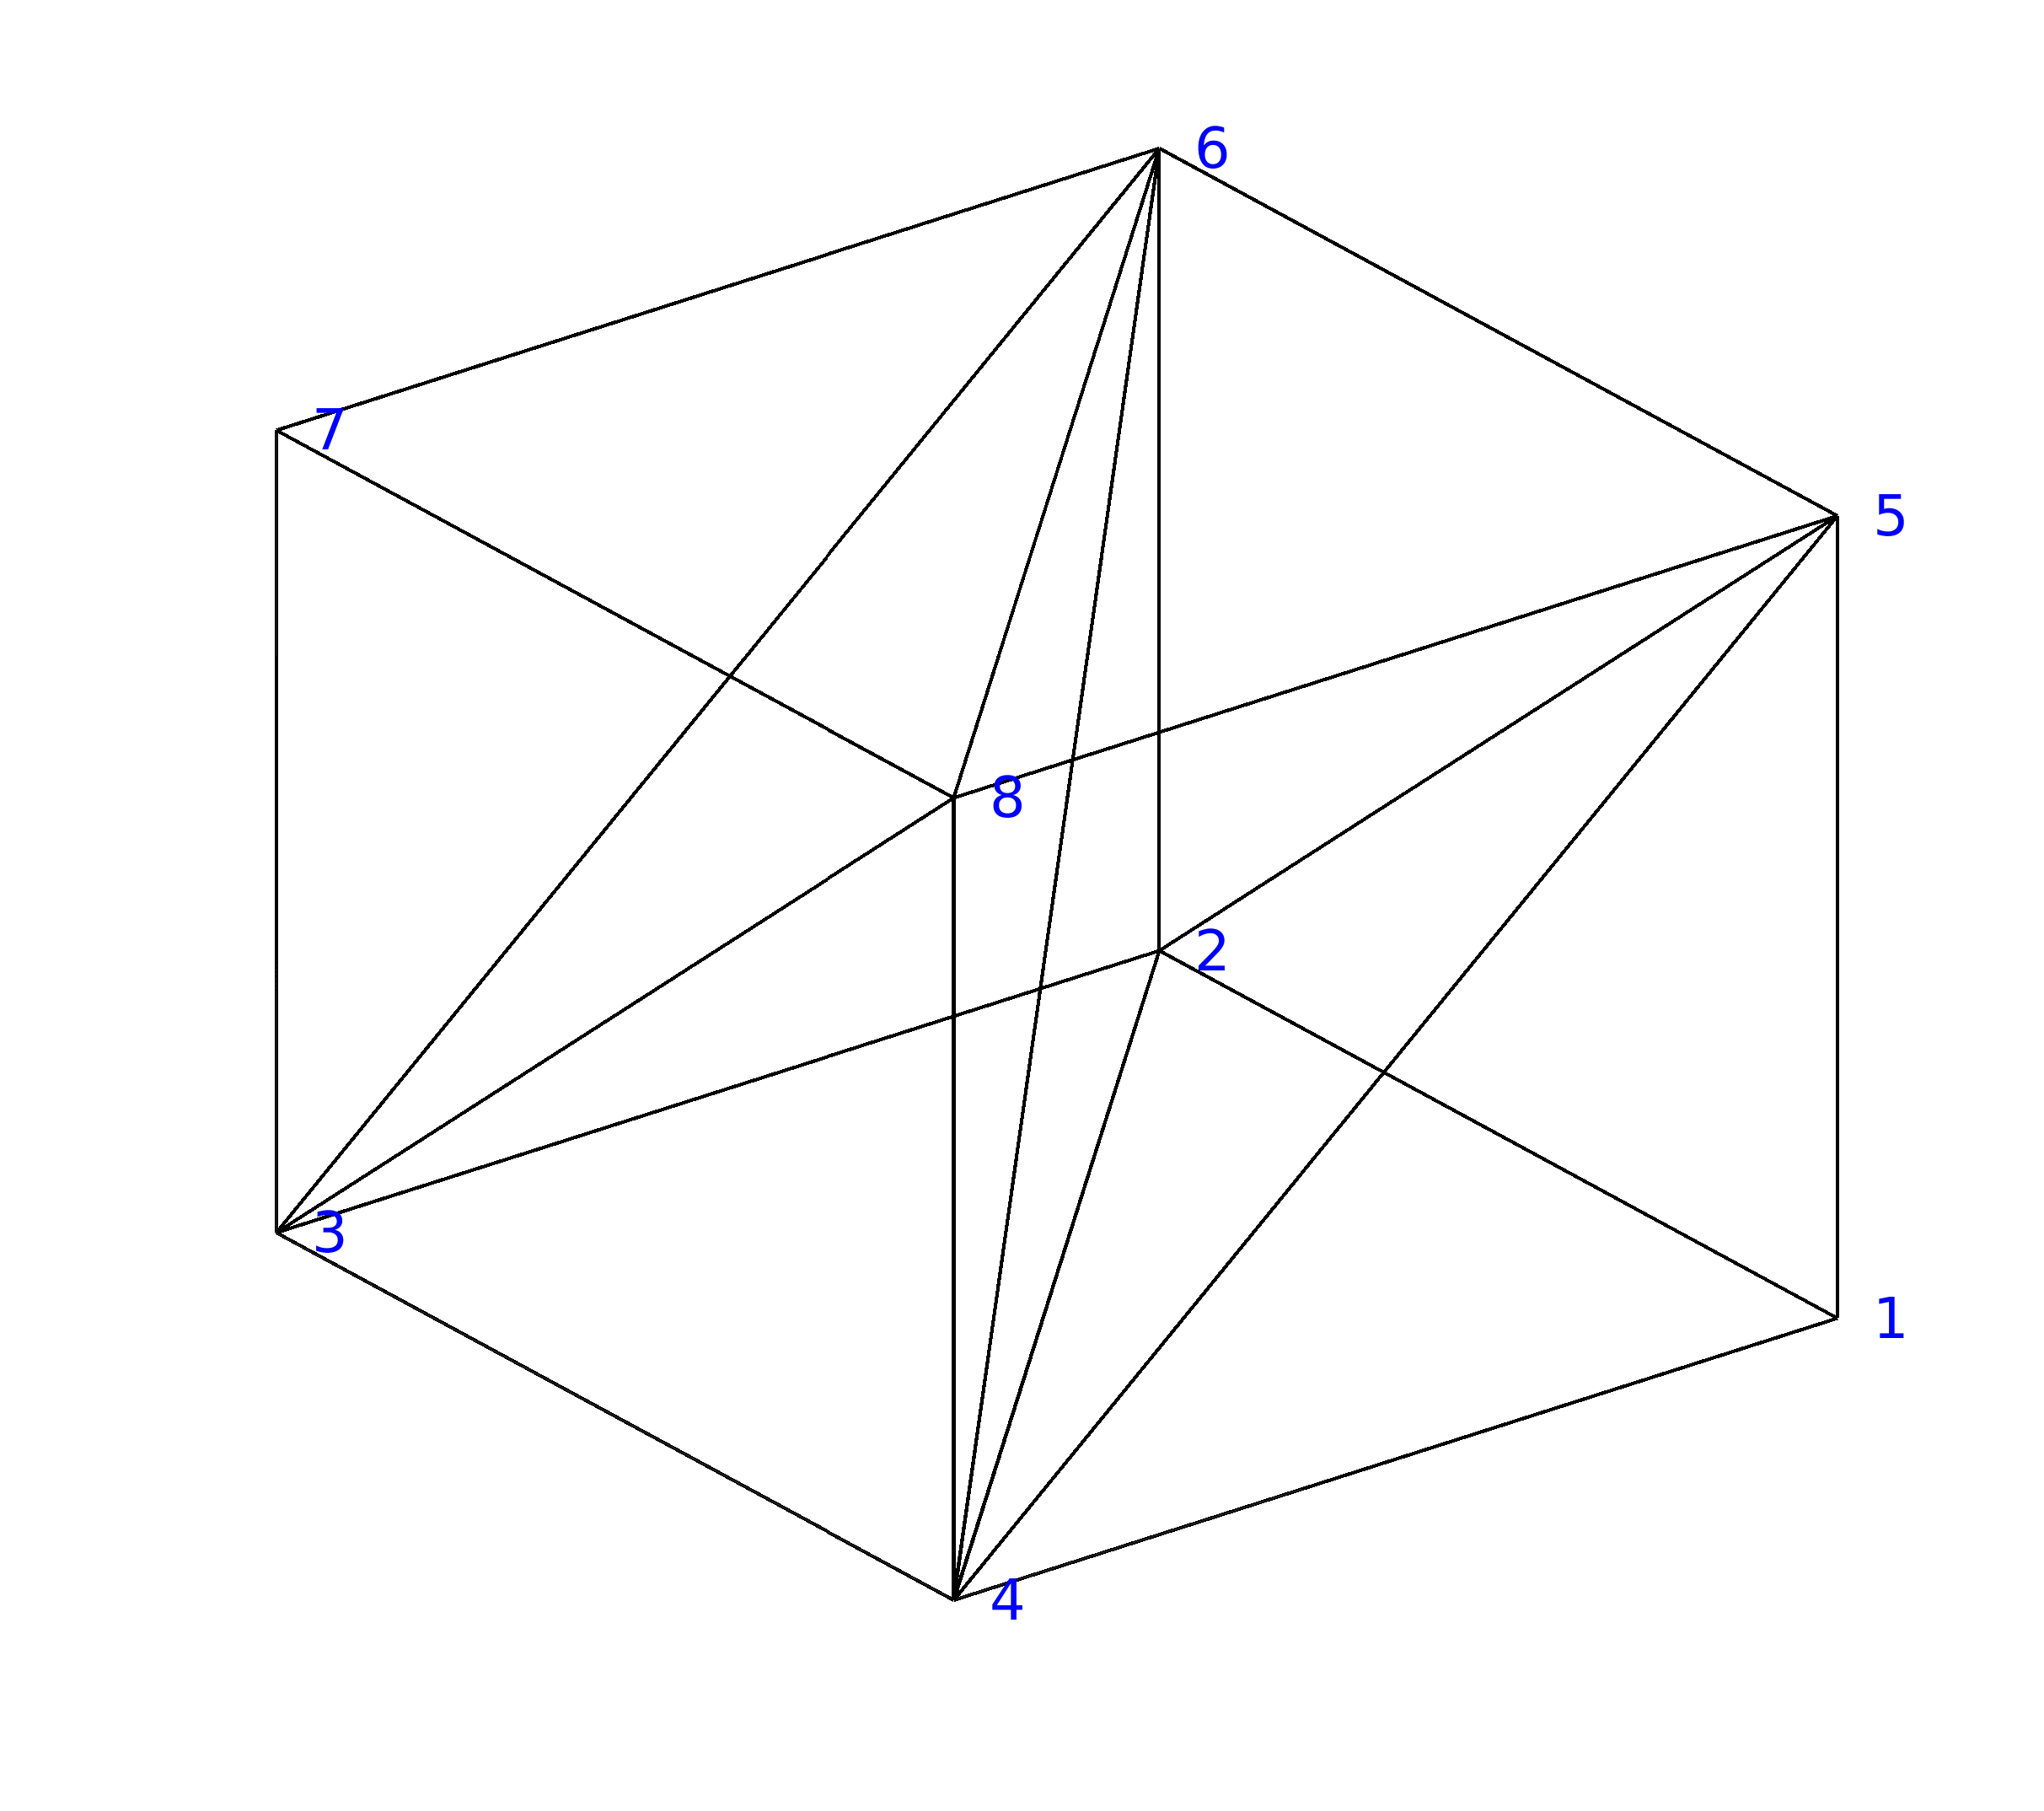
\includegraphics[width=0.8\textwidth]{figures/Tetra_split.eps}
\captionsetup{justification=raggedright,singlelinecheck=false}  
	\caption{Hexahedron split up into six tetrahedra}
	\label{fig:Tetrahedra_in_Cube}
\end{figure}

Here, the plane containing points $(2,4,6,8)$ cuts the hexahedron in half and therefore splits it up into two symmetric prisms. The first prism is then split up into three tetrahedra with the corner points $(1,2,4,5),(2,4,5,6)$ and $(4,5,6,8)$.
The point indices of the tetrahedra of the second prism are $(2,3,4,6),(3,4,6,8)$ and $(3,6,7,8)$, respectively. 

For each direction $(R,\varphi,Z)$ the two faces with respect to that direction have the same orientation of the diagonal intersection of the faces. This means, that these hexahedra can be stacked next to each other in any direction without crossing edges of tetrahedra, as long as the orientations of all hexahedra are the same. 

The indices of all vertices for each tetrahedron can be retrieved by iterating over all hexahedra within the domain using loops over $i,j$ and $k$, transforming the corner points into integer labels using formula \ref{eq:transform_ijk_to_ind} and then saving the correct corner point indices for each of the six types of tetrahedra. Upon generation of each tetrahedron a separate counter that labels the tetrahedra with an integer label needs to be incremented.

By now, all vertices of the grid have been generated, also the vertices have been properly \enquote*{connected} to form tetrahedra that completely fill the domain of the grid.

\subsection{Get neighbors of tetrahedra}
In this section the procedure of finding the indices of neighboring tetrahedra with respect to a given tetrahedron will be explained.\newline
Each tetrahedron can be seen as a part of a hexahedron at position $(i,j,k)$. The indices belonging to the corner points of such a hexahedron are given in section \ref{ssec:getverts} using \ref{eq:transform_ijk_to_ind} while the index of the corner point $(i,j,k)$ can be interpreted as the index of the hexahedron at hand. Since the tetrahedra were labeled in the same order as the hexahedra, there is a simple formula to index all six tetrahedra belonging to a given hexahedron at position $(i,j,k)$:

\begin{eqnarray}\label{eq:ind_tetra}
ind_\text{tetra}(i,j,k,l) = 6(ind_\text{hexa}(i,j,k)-1)+l = \\
\nonumber
= 6(k-1 + (i-1)\cdot N_Z + (j-1)\cdot N_Z\cdot N_R)+l\\
l = 1,2,..,6
\end{eqnarray}

All neighboring tetrahedra must either lie within the same hexahedron as the reference tetrahedron or within a neighboring hexahedron. For this reason it is convenient to use formula \ref{eq:ind_tetra} to obtain the indices of all tetrahedra that are within the same or the neighboring hexahedra. One can then loop over all faces of all tetrahedra and compare the indices of the vertices at the given face of a tetrahedron with the vertices of the faces of all potential neighbors. If three vertices coincide, a matching face and therefore the neighbor to the given face is found. Using this procedure, all tetrahedra can be efficiently connected, by setting the default value for the neighbor indices to $-1$, all border tetrahedra that have no matching neighbor to a face will automatically have set the correct value, as defined in the requirements for the grid.
\subsection{Periodic boundary conditions}
Furthermore, since this grid is constructed using cylindrical coordinates, periodicity in the $\varphi$ coordinate occurs which needs to be treated independently. The issue is that vertices lying on the $\varphi = 0$ plane have both values $0$ and $2\pi$ in the $\varphi$ component and particles that move through the boundary experience a jump in coordinate. Furthermore, since normal vectors must be computed from corner vertices and field quantities are later linearized within the grid, coordinates of corner vertices of all tetrahedra must be smooth with respect to each other and not experience such discontinuities. A possible solution to this problem is to introduce an additional set of vertices, where each element corresponds to a vertex on the $\varphi= 0$ plane but with the $\varphi$ component being shifted to $2\pi$. Neighbor indices can still be obtained by proper indexing, a drawback of this approach however is, that vertices at the periodic boundary plane have different indices on both sides while actually being the same vertex in real space. In case that such information is relevant, this needs to be taken into account independently. While this approach is a working solution, for further grid implementations the approach was changed to not have two indices for any existing vertex. However, here the jump in coordinate needs to be detected upon computation of normal vectors.  
\subsection{Grid visualization}
A full 3D representation of a rather coarse cylindrical contour grid with grid size $(N_R,N_\varphi,N_Z) = (8,16,8)$ is given in figure \ref{fig:full_grid_rect}. Axis orientations are given by the arrows on the top left with the blue arrow indicating the symmetry direction $Z$. Furthermore, one can see that the center region is not part of the grid, this is simply due to range restrictions in $R$ direction as this region is anyway obstructed by the solenoid in a real tokamak and therefore irrelevant for particle guiding center motion. Figure \ref{fig:slice_grid_rect} shows additionally a single $\varphi$ slice of the cylindrical contour grid for better imaginability of intersections at tetrahedra boundaries.

\begin{figure}[h]
	\begin{subfigure}[b]{0.45\textwidth}
		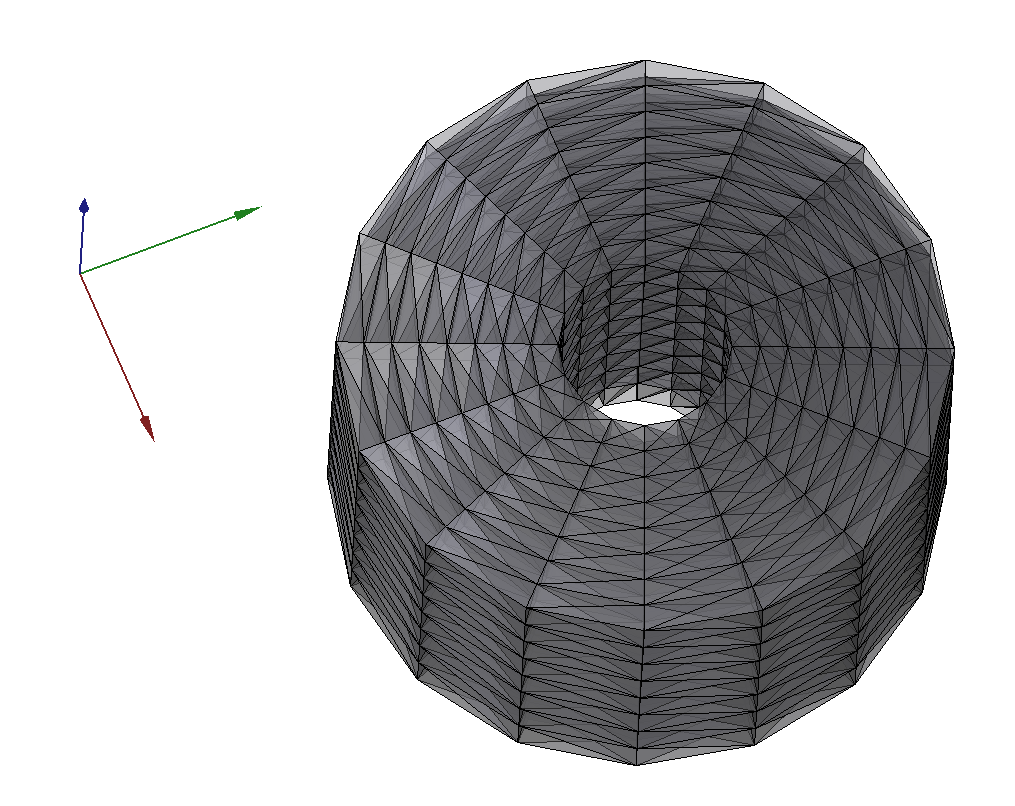
\includegraphics[width=\textwidth]{figures/full_grid_rect.png}
		\caption{Cylindrical contour grid in real space}
		\label{fig:full_grid_rect}
	\end{subfigure}
	\hfill
	\begin{subfigure}[b]{0.45\textwidth}
		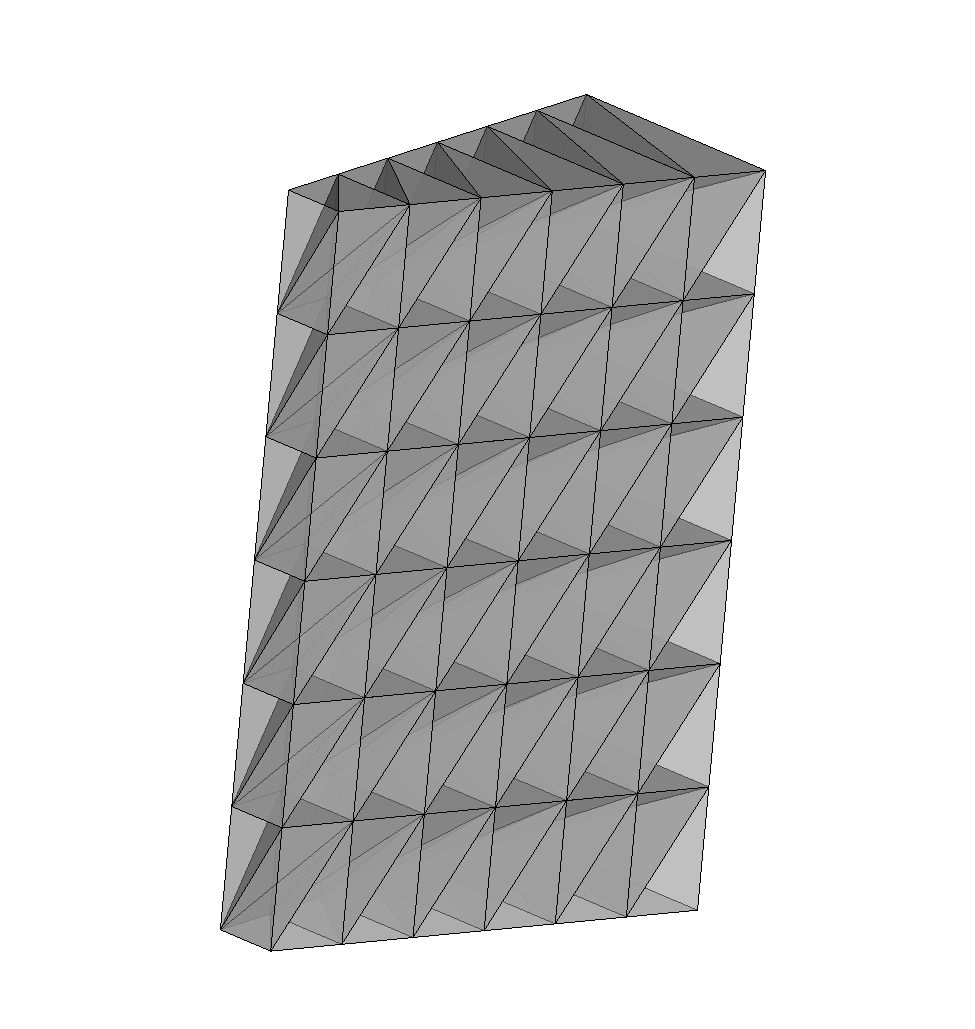
\includegraphics[width=\textwidth]{figures/slice_grid_rect.png}
		\caption{Single $\varphi$ slice of cylindrical contour grid in real space}
		\label{fig:slice_grid_rect}
	\end{subfigure}\hfill
\end{figure}

\subsection{Field lines in cylindrical contour grid using cylindrical coordinates}
Using the cylindrical contour grid for computation of guiding center motion with $GORILLA$ in cylindrical coordinates also allows to easily compute field lines by following electrons at very low energies (it is sufficient to use energies of \SI[prefixes-as-symbols=false]{e-2}{eV}) and strong magnetic fields (magnetic field components are scaled by $1E5$) leading to miniscule larmor radii and a diminishing curvature drift, hence any drift motion becomes negligible. Such a particle will then accurately follow magnetic field lines. If one follows such a particle for a long enough time given that the safety factor $q$ (which is the ratio of number of toroidal turns and number of poloidal turns in a fusion device) assumes an irrational number, a continuous surface will be covered by a single field line. Such a surface is a so-called flux surface where both the poloidal and toroidal magnetic flux remain constant within the central hole of the torus and the toroidal cross section, respectively. One can furthermore intersect a given flux surface with the $\phi=0$ plane to create a Poincar\'e plot. Such plots, calculated using cylindrical coordinates, are given for the cyldrical contour grid in figure \ref{fig:field_lines_rect_grid} and \ref{fig:field_lines_fine_rect_grid}:

\begin{figure}[h]
	\begin{subfigure}[b]{0.5\textwidth}
		\centering
		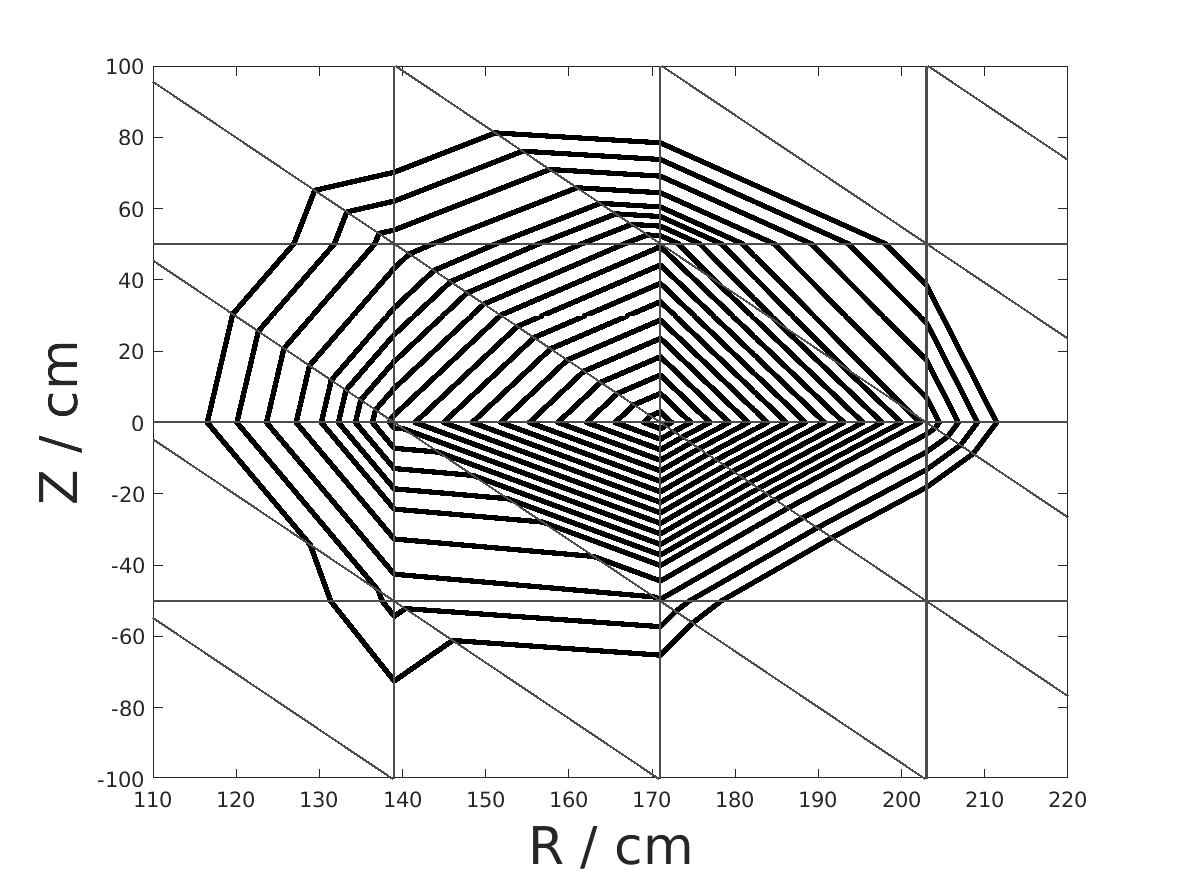
\includegraphics[width=\textwidth]{figures/field_lines_rect_grid.pdf}
		\captionsetup{width=1\textwidth}
		\caption{Poincar\'e cut of flux surfaces calculated with $GORILLA$ using a coarse cylindrical contour grid of $6\times16\times6$}
		\label{fig:field_lines_rect_grid}
	\end{subfigure}
	\hfill
	\begin{subfigure}[b]{0.5\textwidth}
		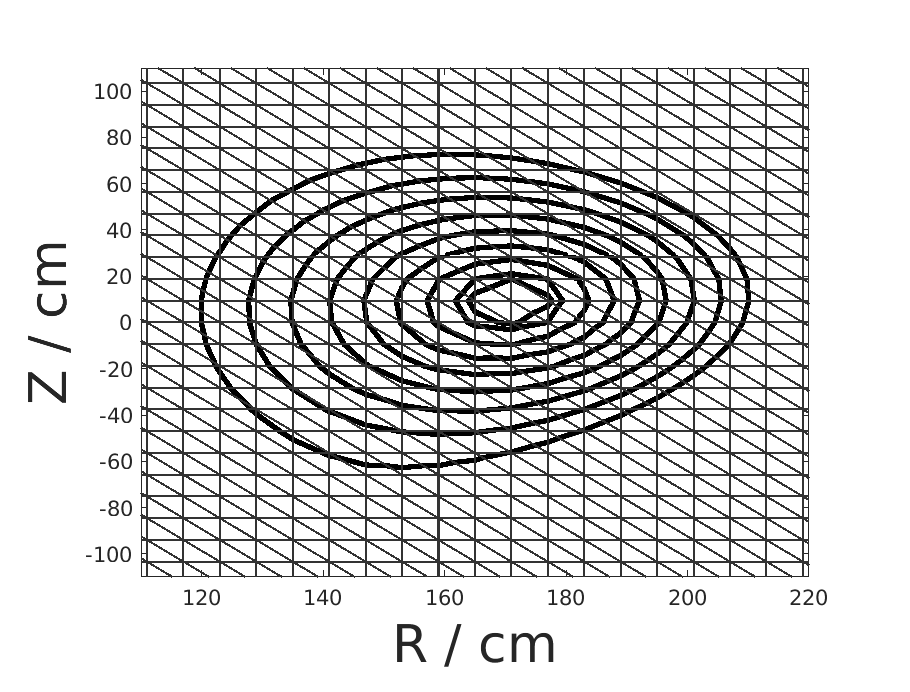
\includegraphics[width=\textwidth]{figures/field_lines_fine_rect_grid.eps}
		\captionsetup{width=1\textwidth}
		\caption{Poincar\'e cut of flux surfaces calculated with $GORILLA$ using a finer cylindrical contour grid of $32\times16\times32$}
		\label{fig:field_lines_fine_rect_grid}
	\end{subfigure}\hfill
\end{figure}





An important fact to note about, regarding these figures, is that due to linearization of field quantities performed by $GORILLA$, all flux surfaces have polygonal shapes. This has to do with the fact, that the field lines in a toroidal configuration, which is used for fusion devices, are curved lines in real space and a linearization in cylindrical coordinates will always introduce an interpolation error leading to polygonally shaped flux surfaces and, thus, also polygonal guiding center orbits of $0^{th}$ order in larmor radius. One can reduce these effects by using a finer mesh, as shown in figure \ref{fig:field_lines_fine_rect_grid}, however this comes at the expense of a larger computational cost.
Furthermore, a large drawback of polygonal field lines is that for 3D (non-axisymmetric) field configurations chaos will be introduced when trying to calculate guiding center orbits. If one wants to keep linearization of field quantities for simplicity of equations and, thus, performance reasons, a possible solution to this problem is given via appropriate coordinate transformations where field lines assume straight lines. The use of symmetry flux coordinates (SFC) satisfies such a condition \cite{haeseleer}, however, the cylindrical contour grid will no longer be guaranteed to not have overlaps between tetrahedra, when vertices are directly connected in SFC. Since not having overlaps was one of the initial requirements, a new grid with a more appropriate toroidal shape needs to be implemented for the use of SFC.

%\section{Circular Grid}
%\subsection{Delaunay Triangulation}
%\subsection{2D part}
%\subsection{3D part}

\section{Field Aligned Grid}
One is now interested in computing guiding center orbits in symmetry flux coordinates (SFC) where field lines are represented by straight lines. The straightness of field lines in these coordinates allows to compute guiding center motion also for generally non-axisymmetric field configurations without introducing artificial chaos. Furthermore, field lines calculated in SFC will coincide more accurately with physical field lines, compared to when calculated in cylindrical coordinates where they assume polygonal shapes. A problem that arises by using SFC is, however, that in SFC the cylindrical contour grid is no longer guaranteed to satisfy the requirement that tetrahedra must not overlap. Therefore, a new grid with a field aligned geometry is needed. Such a grid can be obtained by positioning the grid vertices equidistantly along the coordinate contours of $(s,\vartheta_f,\varphi)$, where $s$ denotes the normalized flux label (normalized poloidal or toroidal flux), $\vartheta_f$ the symmetry flux poloidal angle and $\varphi$ the toroidal angle, respectively. With such an approach, only a routine is needed that transforms any given point in SFC back to cylindrical coordinates, where physical field quantities are available. It should be furthermore pointed out, that any grid generated by setting equidistant points in three dimensions will be topologically identical to the cylindrical contour grid in cylindrical coordinates, thus an analogous indexing scheme for tetrahedra can be applied. In this section, an approach to obtain a routine that converts given SFC coordinates to cylindrical coordinates for an axisymmetric field configuration is explained. A different code package for stellarator configurations has been made available by Sergei Kasilov and has been implemented in the $GORILLA$ code. In this thesis only the axisymmetric approach will be discussed. 

\subsection{Field lines in toroidal fusion devices and safety factor}
When trying to construct a field aligned grid, one must first look at the geometry of magnetic field lines themselves. By definition, magnetic field lines are curves of which the tangent is always parallel to the magnetic field vector \cite{haeseleer}. Mathematically this translates to the set of differential equations
\be{eq:fieldlines}
\frac{\textrm{d}R}{\textrm{d}\varphi} = \frac{B^R}{B^\varphi}, \hspace{0.1cm} \frac{\textrm{d}Z}{\textrm{d}\varphi} = \frac{B^Z}{B^\varphi},
\ee

where $(R,\varphi,Z)$ denote cylindrical coordinates and $(B^R,B^\varphi,B^Z)$ the contravariant components of the magnetic field. Important properties of field lines are that they always remain closed and cannot cross other field lines. Furthermore, the absolute strength of the magnetic field at a given point is proportional to the number of field lines going through an infinitesimal area located at that point and perpendicular to the magnetic field vector, thus it is proportional to the areal field line density.\newline
By numerical integration of set \ref{eq:fieldlines} over $\varphi$ for some arbitrary starting position using a standard ordinary differential equation solver (e.g. $RK45$), a field line can be traced.
In toroidal fusion devices when tracing such a field line associated with a given starting position for one toroidal turn, in general one does not reach the same point in space but rather a different location in the poloidal plane at the starting toroidal angle. The different rates of change in coordinates $(\vartheta,\varphi)$ per toroidal turn are hereby linked by the safety factor 

\be{eq:safetyfactor}
q = \frac{B^\varphi}{B^\vartheta} \hspace{0.4cm}\text{to}\hspace{0.4cm} \textrm{d}\varphi= q\textrm{d}\vartheta.
\ee

For irrational values of $q$, this field line will completely fill a 2-dimensional surface which is then called flux surface, as both toroidal and poloidal magnetic flux remain constant within a given field line. By gradually changing the starting point of integration for field lines towards the center of a corresponding flux surface in the poloidal plane, one can asymptotically reach a degenerate flux surface which is represented by a single line, this field line is called the magnetic axis and will be used for the point of origin in s-direction for symmetry flux coordinates. For the use of SFC, one must assume that only one magnetic axis exists with all flux surfaces being nested flux surfaces, thus no magnetic islands are allowed.
The outermost closed flux surface is called the separatrix, marking the transition between core plasma region and the scrape-off layer. In this thesis, only the core plasma region is considered, additions to the grid must therefore be programmed if one wants to include the scrape-off layer into calculations.

Figure \ref{fig:field_lines_torus} shows some schematic field lines in a tokamak for different values of $q$, each for one poloidal turn. As can be seen, only field lines with integer valued $q$ are closed after one poloidal turn. 

\begin{figure}[h]
	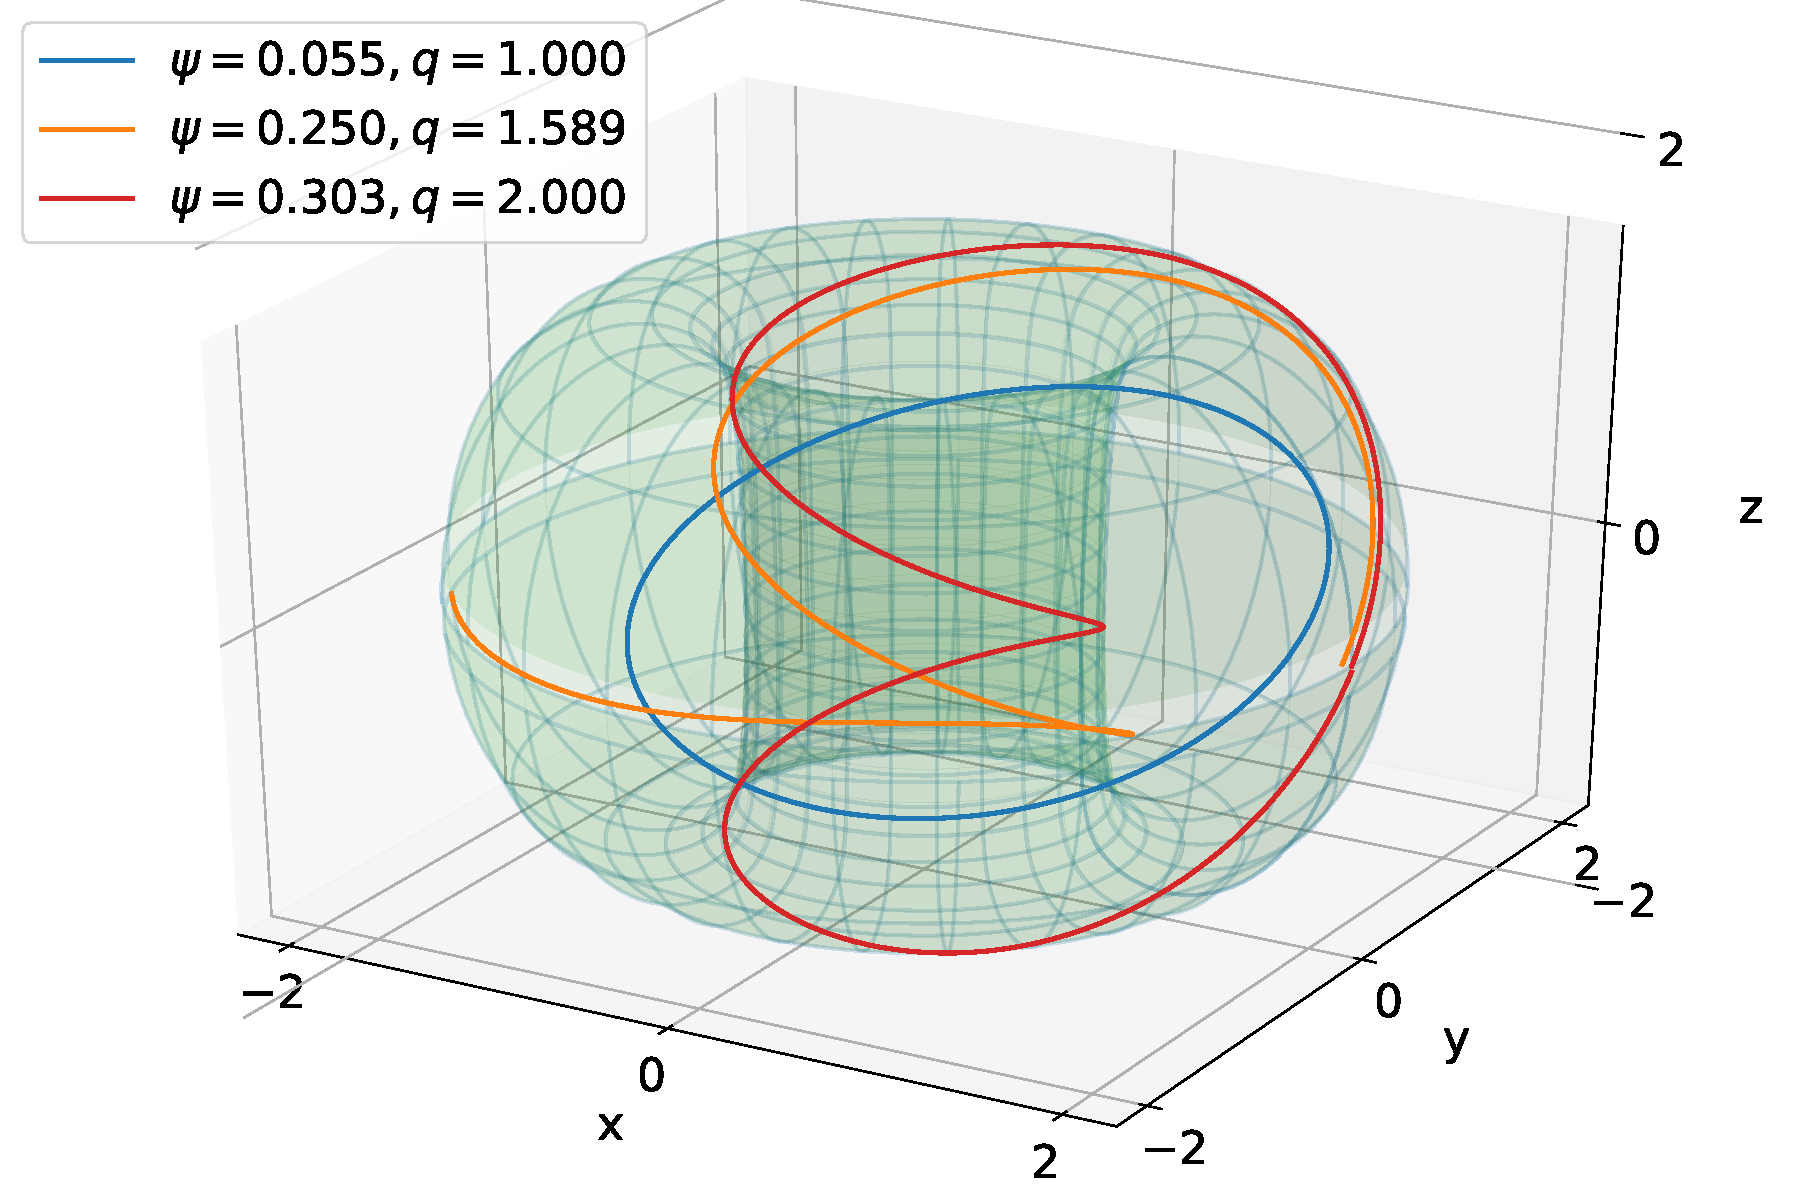
\includegraphics[width=0.9\textwidth]{figures/field_lines_torus.pdf}
	\caption{Field lines with different safety factors in a tokamak}
	\label{fig:field_lines_torus}
\end{figure}



\subsection{Field line integration and splining of axisymmetric fields}
Next, one wants to construct a routine to map symmetry flux coordinate triplets to cylindric coordinates, in which all field quantities are subsequently read out.
The approach presented here is only applicable for axisymmetric field configurations, as present in ideal $Tokamaks$.
 Symmetry flux coordinates topologically represent toroidal coordinates, therefore the first SFC coordinate is a minor radius-like quantity $s$, which in our case is chosen to be the normalized toroidal flux. However, in theory any flux label can be used, the second coordinate is $\vartheta$ which is related but not identical to the geometrical poloidal angle $\theta$. The last coordinate is the geometric toroidal angle $\varphi$, which is the same as in standard cylindrical coordinates. Since field lines are chosen to be straight in these coordinates, the simple relation that the change in $\vartheta$ along the field line is proportional to the change in $\varphi$ must hold, this proportionality factor represents the safety factor shown above. Hence, if one performs a step-wise integration of equation set \ref{eq:fieldlines} equidistantly along $\varphi$ from 0 to $q2\pi$ and calculates these points in $(R,\varphi,Z)$ they must automatically correspond to point sets $(s,\vartheta,\varphi)$ with s being constant along a field line (0 at the magnetic axis and 1 at the separatrix), $\vartheta$ being equidistant from 0 to $2\pi$ and $\varphi$ being equidistant from 0 to $q2\pi$. For an axisymmetric configuration, one can now convert these coordinates to cylindrical coordinates via interpolation. A more detailed explantion of the procedure is given below.


\subsubsection{Find O-point (magnetic axis)}
The first step in implementing SFC is to find the magnetic axis which represents the $s=0$ flux surface. This is done by starting to integrate a field line  at position $(R,\varphi,Z) = (\frac{1}{2}(R_{min}+R_{max}),0,\frac{1}{2}(Z_{min}+Z_{max}))$. The corresponding field values are obtained from calling the $field$ routine that returns all necessary field information for the configuration. From this starting position the field line is intergrated for one toroidal turn using a standard ODE solver. Apart from the set of ODE for the magnetic field line, also the $R$ and $Z$ coordinates are computed independently by the ODE solver. From this information, one can directly calculate the mean values of $R$ and $Z$ when following the field line by dividing the integrated values of $R$ and $Z$ by the integration angle of $2\pi$. These values are then used for the next guess for the magnetic axis. From this new starting point another field line is followed and the mean values of $R$ and $Z$ are again computed. This iteration quickly converges to the position of the magnetic axis for a toroidally symmetric field. This routine is implemented in the file \texttt{field\_line\_integration\_for\_SYNCH.f90} where by default 20 iterations are performed.
\subsubsection{Find X-point}
Now that the magnetic axis has been found, the innermost starting point in the $\varphi = 0 $ plane for the field line integrations has been determined. The outermost starting point will be given by a point on the separatrix, which is the boundary between closed and open flux surface domains (i.e. core region and scrape-off layer). To find a starting position on the separatrix, one takes the coordinates of the magnetic axis and parametrizes a line segment in cylindrical $R$-direction up to the largest $R$-value possible (saved in \texttt{rmx}) for the given configuration. The boundaries of $R$ and $Z$ for the current configuration are saved within the module \texttt{field\_eq\_mod} in file \texttt{field\_divB0.f90} and can be read out via

\texttt{rmn=rad(1)\\
rmx=rad(nrad)\\
zmn=zet(1)\\
zmx=zet(nzet)}.

This line segment is then split up equidistantly, by default 10000 points are chosen. Points $p_i$ are placed equidistantly with
\be{eq:points_ox}
\vec{p_i} = \vec{\text{O}} + \frac{i}{N}\begin{pmatrix}rmx-O_R\\0\end{pmatrix}
\ee
in cylindric coordinates for $i = 0,1,2,..,N$. Now, starting from the magnetic axis, for each of these points a magnetic field line is integrated for two poloidal half turns in successive steps of $\Delta\varphi=2\pi/10$, resulting in one full turn. After each integration step the current position is compared to the $(R,Z)$-constraints of the domain, in case a maximum/minimum value is exceeded the current field line is no longer closed. Thus, the previous starting point for the integration can be assumed to represent the starting point for the last flux surface. However, this last closed field line is already suboptimal in quality so the preceding starting point is taken as the last closed field line for this configuration, hence representing the separatrix. As mentioned above, the X-point lies on the separatrix, in addition to this condition, the X-point has the property that the poloidal magnetic field vanishes at its position. Consequently, when following the last closed field line, upon reaching the X-point no poloidal movement occurs, thus $(R,Z)$ remain constant.
The algorithm for finding the X-point uses this property by integrating the last closed field line in steps of $\Delta\varphi=2\pi/10$ and comparing the last $(R,Z)$ position with the position of the previous integration step. The distance between the two positions is evaluated and compared with the distance between the positions of the previous steps, if the new distance is so far the lowest, the new position and the distance are saved in variables \texttt{min\_d} and \texttt{x\_point}. These steps are performed until the distance between steps no longer decreases, the position of the X-point is hereby found. To make sure that one only integrates over one poloidal turn, one can use the property of the cross product that $|\vec{a}\times\vec{b}| = |a||b|\sin(\alpha)$ with $|\vec{a}|$ being the poloidal starting position of the integration and $|\vec{b}|$ the current poloidal position. Upon completing one full poloidal turn, the sign of the sine will flip from -1 to 1, by detecting this flip one can stop the integration accordingly.  


% The value of the normalized flux label $s$ is chosen to be 1 at the separatrix (in this application $s$ represents the toroidal magnetic flux enclosed in a flux surface, divided by the total toroidal magnetic flux at the separatrix, but generally any flux function can be used). The point on the separatrix where the flux surface intersects with itself is called the X-point. Furthermore, for symmetry flux coordinates the $\vartheta=0$ contour can be freely chosen. For this application this contour will be parametrized to be a straight line in cylindrical coordinates (this line is set to be straight in symmetry flux coordinates as well) going from the magnetic axis to the X-point in the $(s,\vartheta)$ plane. The coordinate system is now fully defined. 

\subsubsection{Scanning flux surfaces}
After finding the O-point and the X-point, the next step is to connect them by a straight line in cylindrical coordinates in the $\varphi=0$-plane, this line segment is subsequently chosen to respresent the $\vartheta=0$ contour in SFC. On this line segment 500 points are placed equidistantly, then for each of these points, an independent field line integration over one poloidal turn with a step size of $\Delta\varphi=2\pi/10$ is started. The goal of these particular integrations is to determine the safety factors of the individual field lines, which can be easily calculated from the toroidal integration angles corresponding to exactly one poloidal turn. Again, the approach using the flip of the cross product sign will be used to determine whether the last integration step finished the turn. However, due to the finite size of the integration steps the necessary toroidal integration angle is not precisely determined. Thus, iterations of Newton's method are applied in order to obtain the precise integration angle to complete the turn. To implement such a routine, one needs to take a look at some geometric considerations. Figure \ref{fig:field_line_integration_geometric} depicts a sketch of the components relevant for Newton's method:

\begin{figure}[h!]
	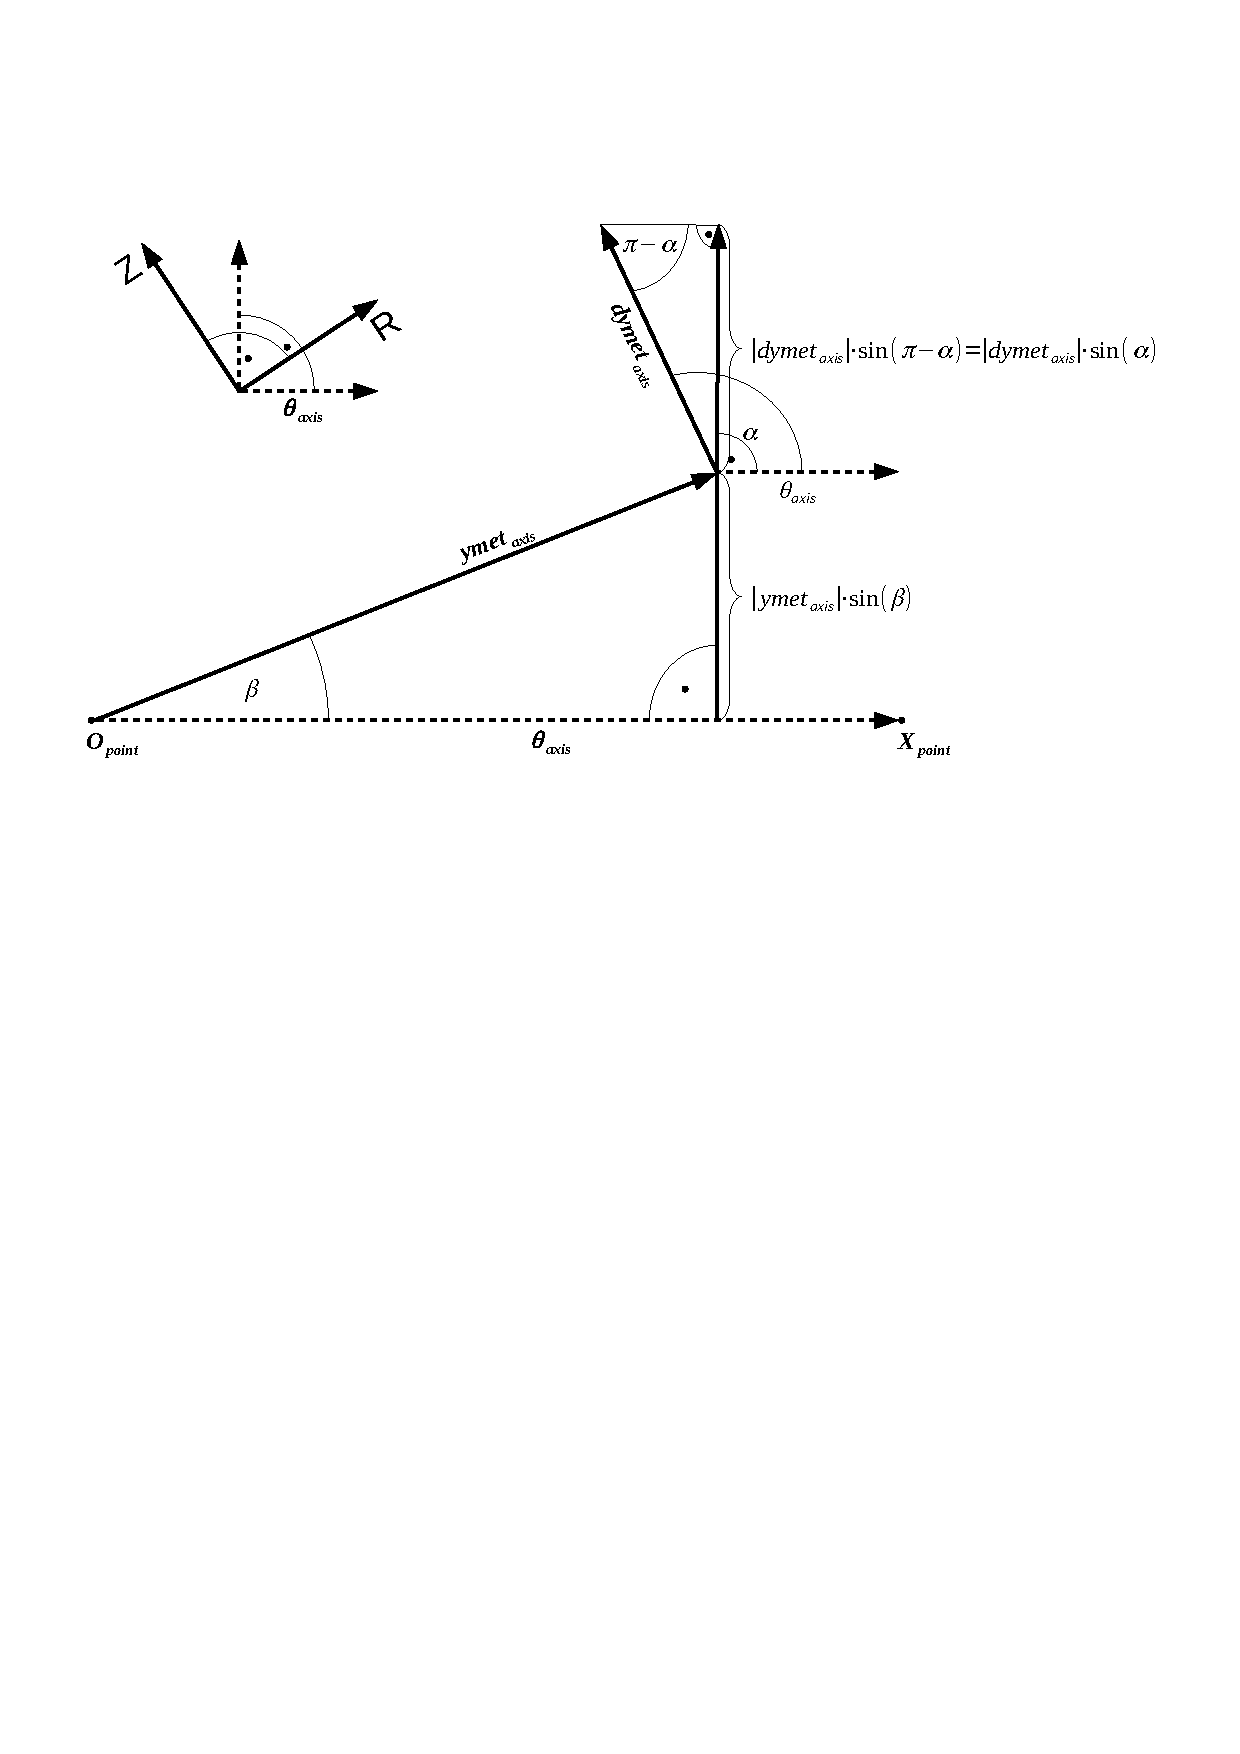
\includegraphics[trim={5 15cm 0 5},clip, width = 1.0\textwidth]{figures/fli_angle_graphics.pdf}
	\caption{Visualization of quantities for Newton's method}
	\label{fig:field_line_integration_geometric}
\end{figure}

In order to implement a Newton's scheme, one first takes a look at the normal distance from the position after the last integration step $ymet_\text{axis}$ to the $\theta=0$ axis, for this it is convenient to rotate the system such that the $\theta$ axis points in the $x$-direction. The normal distance from the end position $\bm{ymet_\text{axis}}$ to the axis $\bm{\theta_\text{axis}}$ is then given by 
\begin{equation*}
	d_\perp =|\bm{ymet_\text{axis}}|\sin(\beta).
\end{equation*}
Next, one is interested in the normal derivative of the field line to the axis with respect to $\varphi$. In the routine, the derivatives $dr\_dphi$ and $dz\_dphi$ are provided by the numerical integration scheme, here they are combined in vector $\bm{dymet_\text{axis}}$. Using the identity $sin(\pi-x)=sin(x)$ one can evaluate the normal derivative as 
\begin{equation*}
\frac{\partial d_\perp}{\partial \varphi} =|\bm{dymet_\text{axis}}|\sin(\alpha),
\end{equation*}
with Newton's guess for the correction of the integration angle

\begin{equation*}
\Delta\varphi=\sigma\frac{d_\perp}{\left(\frac{\partial d_\perp}{\partial \varphi}\right)} = \sigma\frac{|\bm{ymet_\text{axis}}|\sin(\beta)}{|\bm{dymet_\text{axis}}|\sin(\alpha)}
\end{equation*}

and $\sigma$ being the sign of $(\bm{ymet_\text{axis}} \times \bm{\theta_\text{axis}})$ to ensure the correct direction of integration. This correction scheme is applied iteratively for each field line, by default 50 iterations are performed to obtain accurate values for $\varphi_\text{total}$.

Upon determining the correct toroidal integration limits to complete one poloidal turn for each point, the safety factors for the field lines are then directly given by
\begin{equation*}
q_\text{saf} = \frac{\varphi_\text{total}}{2\pi}.
\end{equation*}

Apart from the safety factor, also the approximate average minor radius of the field line \texttt{rsmall}, the poloidal flux $\psi_\text{surf}$ (variable \texttt{psisurf}) and the toroidal flux $\Phi_\text{tor}$ (variable \texttt{phitor}) are computed for each field line. For the application at hand \texttt{rsmall} is irrelevant so it will not be discussed, \texttt{rbeg} is also an output of the routine which has no physical meaning as it is never evaluated (it is not removed to ensure that the function call stays the same for compatibility with other codes), the poloidal flux $\psi_\text{surf}$ is obtained from the module \texttt{field\_eq\_mod} by calling the \texttt{field\_eq} subroutine at the start position of the integration, from this value the poloidal flux at the magnetic axis then needs to be subtracted (its value is computed also via the \texttt{field\_eq} subroutine). The toroidal flux \texttt{phitor} is calculated by numerically integrating equation 
\begin{equation*}
\frac{\partial \Phi_\text{tor}}{\partial \varphi} = R\cdot Z\cdot B_r  
\end{equation*}
when performing the field line integration, here $B_r$ denotes the physical component of the magnetic field in the $R$-direction. For normalization, the obtained result still needs to be divided by $2\pi$. 

So far, the flux functions \texttt{rsmall}, \texttt{qsaf}, \texttt{psisurf} and \texttt{phitor} were calculated for the array of 500 field lines, with flux functions being defined as functions that remain uniform along a field line / on a flux surface, thus only depending on the flux surface label. Due to this property any flux function can be used to label a given flux surface, in this application the normalized toroidal magnetic flux, here denoted \textit{s}, will be used as the flux label. Now, one is interested in the positions $R$, $Z$, the modulus of the magnetic field \texttt{bmod}~$=(|\mathbf{B}|)$ and the metric determinant \texttt{sqgnorm}~$=(\sqrt{|g|})$ in equidistant steps along the field lines. These values are needed for the interpolation routine to convert components from symmetry flux coordinates to cylindric coordinates.
Due to axisymmetry in the configuration the field lines only need to be integrated for exactly one poloidal turn, so all field lines need to be integrated for the previously found $\varphi_{total}$ values in $\varphi$ direction over 500 equidistant steps. After each step, $R$ and $Z$ are obtained directly as output argument from the standard ODE integrator, physical components of the magnetic field are obtained from calling the \texttt{field\_eq} routine, thus \texttt{bmod} ~$= \sqrt{B_r^2+B_p^2+B_z^2}$, finally \texttt{sqgnorm} for symmetry flux coordinates is calculated via \texttt{sqgnorm}~$ = R/|B_p|$. 

On a sidenote, due to the straightness of field lines in symmetry flux coordinates the points along the field lines are equidistant in both $\varphi$ and $\vartheta$ but generally not in $s$ direction, however $s$ remains constant along a given field line.

\subsubsection{Interpolation of data with respect to $\vartheta$ and normalization}
The algorithms concerning field line integration which are explained in the previous subchapters are all part of the same subroutine \texttt{field\_line\_integration\_for\_SYNCH}. This subroutine is called from a second subroutine \texttt{preload\_for\_SYNCH} where the calculated quantities are saved into separate files. These files are subsequently read out from a third subroutine \texttt{load\_magdata\_in\_symfluxcoord}. In this subroutine, the data for each field line is then interpolated with periodic third order splines in theta with the subroutine \texttt{spl\_per}, the toroidal angle is no longer of interest due to axisymmetry as it is equivalent to the toroidal angle in cylindric coordinates. Moreover, since for each field line the flux label $s$ remains constant, the change of each quantity along a given field line must be purely a function of the symmetry flux coordinate $\vartheta$. The spline coefficients from the \texttt{spl\_per} subroutine are then saved into variables \texttt{R\_st}, \texttt{Z\_st}, \texttt{bmod\_st}, \texttt{sqgnorm\_st} (suffix \texttt{\_st} stands for splined in theta). The calculated flux functions are then also read out from the file, however, these quantities remain constant along the field line so there is no need for splines in $\vartheta$ direction. Since only the normalized fluxes are of interest for this application, both $\psi_{surf}$ and $\Phi_{tor}$ are divided by their maximum values. The normalized toroidal flux $s$ will label the individual flux surfaces. 
The precomputed data from \texttt{load\_magdata\_in\_symfluxcoord} are directly saved into the module \texttt{magdata\_in\_symfluxcoor\_mod} since they only need to be precomputed once. The subroutine \texttt{magdata\_in\_symfluxcoord\_ext} then accesses these data and performs the necessary $s$ interpolation for arbitrary positions, which is very efficient compared to the precomputation. 
\subsubsection{s interpolation of data}
In \autoref{chap:AppendixA}, the method of Lagrange polynomial interpolation is introduced. Now to interpolate the data for a given point $(s,\vartheta)$ one searches the field line array via bisection to find the indices and $s$ values of the closest four field lines to the position $s$. As mentioned, this is done in subroutine \texttt{magdata\_in\_symfluxcoord\_ext(inp\_label,s,psi,theta,}\\
\texttt{q,dq\_ds,sqrtg,bmod,dbmod\_dtheta,R,dR\_ds,dR\_dtheta,Z,dZ\_ds,dZ\_dtheta)},\\
whereby depending on the value of the input label \texttt{inp\_label}, either the variable \texttt{s} or \texttt{psi} define the input for the minor radial position while the variable \texttt{theta} defines the symmetry flux poloidal angle, the toroidal angle \texttt{phi} remains invariant, thus, it is not included in the subroutine call, the remaining arguments are outputs of the subroutine. An overview of the parameters is given in table \ref{tab_input_magdata}. 

The splines for these four field lines are then evaluated for the given $\vartheta$ position, this yields an array of four $s$ values, which are belonging to the field lines, and the corresponding interpolation quantities. With the four $s$ values of the closest field lines, the Lagrange coefficients $\mathscr{L}_k(s)$ are now fully determined, acting as weights for the quantities on the fields lines that are to be interpolated.
The output is then given by

\begin{equation*}
		P(s) = \sum_{k=0}^{n} \mathscr{L}_k(s)f_k
\end{equation*}

for any interpolated quantity $f$. $P(s)$ hereby interpolates $f(s)$ and $f_k$ represents $f(s_k)$ with discrete values $s_k$ at flux surface $k$.


\begin{centering}
	\begin{table}[H]
		
		\caption{Parameters for \texttt{magdata\_in\_symfluxcoord\_ext}}
		\begin{tabular}{|l|l|}
			\hline
			\rowcolor{lightgray}
			Name; Data type&Description \\
\hline
			\multirow{15}{0pt}\newline
			\texttt{inp\_label}; \texttt{integer}& input switch, where 1 sets 					\texttt{s}\\ 
			 & and 2 sets \texttt{psi} as input \\ 
\hline
			\texttt{s}; \texttt{double precision}& normalized toroidal flux, also 				the value of the first\\ 
			&component in SFC (symmetry flux coordinates)\\ 
\hline
			\texttt{psi}; \texttt{double precision}&poloidal flux at $(s,\vartheta,				\varphi)$ \\
\hline  
			\texttt{theta}; \texttt{double precision}& value of the second 						component in SFC \\
\hline
			\texttt{q}; \texttt{double precision} 		 & safety factor at $(s,				\vartheta,\varphi)$\\
\hline
			\texttt{dq\_ds}; \texttt{double precision} & partial derivative of the 				safety factor with respect\\
			& to \textit{s} at $(s,\vartheta,\varphi)$ \\
\hline
			\texttt{sqrtg}; \texttt{double precision} 		 & square-root of the 				metric determinant at $(s,\vartheta,\varphi)$\\
\hline
			\texttt{bmod}; \texttt{double precision} 		 & modulus of the 					magnetic field at $(s,\vartheta,\varphi)$  \\
\hline
			\texttt{dbmod\_dtheta}; 		 & partial derivative of the modulus of 			the magnetic\\
			\texttt{double precision}& field with respect to $\vartheta$\\
\hline
			\texttt{R}, \texttt{dR\_ds}, \texttt{dR\_dtheta};& first component of 				position in cylindric coordinates\\
			\texttt{double precision} & $(R,\varphi,Z)$ and its derivatives with 				respect to \textit{s} and $\vartheta$\\
\hline
			\texttt{Z}, \texttt{dZ\_ds}, \texttt{dZ\_dtheta}& third component of 					position in cylindric coordinates\\
			\texttt{double precision} & $(R,\varphi,Z)$ and its derivatives with 				respect to \textit{s} and $\vartheta$\\
\hline
		\end{tabular}
		\label{tab_input_magdata}	
	\end{table}
\end{centering}

\subsection{Field aligned grid generation}
So far, the subroutine \texttt{magdata\_in\_symfluxcoord\_ext(inp\_label,s,psi,theta,q,dq\_ds,\\sqrtg,bmod,dbmod\_dtheta,R,dR\_ds,dR\_dtheta,Z,dZ\_ds,dZ\_dtheta)} has been constructed to convert arbitrary SFC positions $(s,\vartheta,\varphi)$ back to cylindrical coordinates positions $(R,\varphi,Z)$. Now, the logical scheme that is used in $GORILLA$ for generating the field aligned grid is explained. Here, the subroutines that are called in order to generate the grid are structured according to figure \ref{fig:make_tetra_grid_code_structure}. 

\begin{figure}[H]
	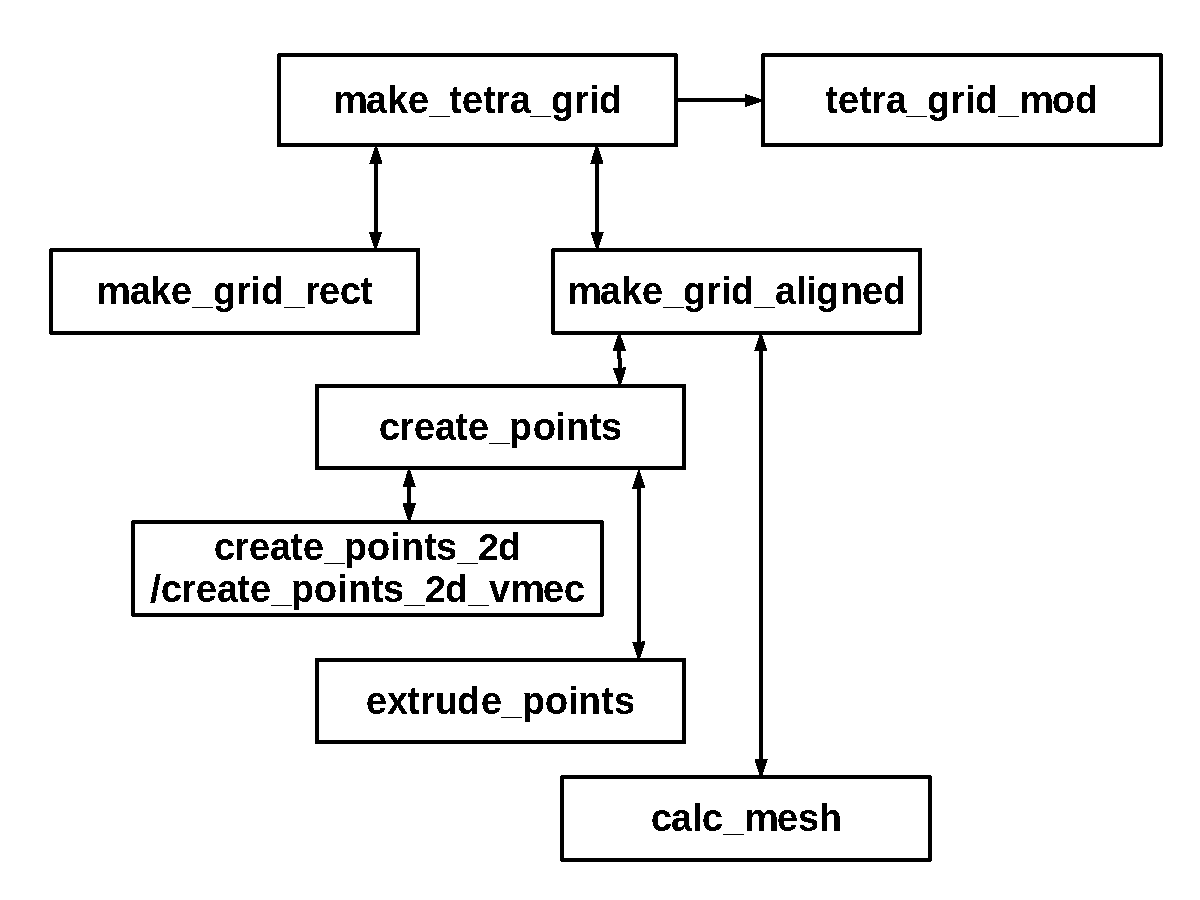
\includegraphics[width=1.0\textwidth]{figures/make_tetra_grid_graphics.pdf}
	\caption{Subroutine \texttt{make\_tetra\_grid} code structure}
	\label{fig:make_tetra_grid_code_structure}
\end{figure}

In this hierarchy, the first subroutine \texttt{make\_tetra\_grid} is called with arguments \texttt{(grid\_kind\_in, grid\_size\_in)}, the first input being an integer label with value 1 for the cylindrical contour grid and 2 for the field aligned grid, the second input is an integer array with 3 elements defining the number of grid elements along each coordinate. From a programmatic aspect, this routine can be thought of as a constructor from object oriented programming as it constructs an instance of a suitable grid according to the Fortran type \texttt{tetrahedron\_grid} (which can essentially be seen as a class) with additional variables saved together in the module \texttt{tetra\_grid\_mod}. In this module, all geometry related properties of the grid are saved, moreover, they are saved with attributes \texttt{public, protected}, thus, while being publically avaiable for read-out they can only be altered from subroutines and functions belonging to the module itself. For this reason the subroutine \texttt{make\_tetra\_grid} must also be defined within the module. By having the entire grid generation being covered with a single subroutine call and not being able to change it otherwise, this adds an additional layer of security regarding unexpected changes of grid quantities due to unintended coding mistakes. 
Depending on which grid one wants to generate (i.e. either the cylindrical contour or the field aligned grid), subsequently either the subroutine \texttt{make\_grid\_rect(tetra\_grid,verts\_rphiz,grid\_size,Rmin,Rmax,Zmin,Zmax)} or the subroutine \texttt{make\_grid\_aligned(grid\_size,efit\_vmec)} is called from \texttt{make\_tet\\ra\_grid}. For the \texttt{make\_grid\_rect} subroutine, the first two arguments denote the output, the latter arguments are inputs for the grid generation. The \texttt{make\_grid\_aligned} subroutine only takes input arguments, as it writes the generated grid data directly into the module, thus, the subroutine must be also defined within the module \texttt{tetra\_grid\_mod}.
For clarity, the elements of the Fortran module \texttt{tetra\_grid\_mod} and type \texttt{tetrahedron\_grid} are displayed in tables \ref{tab_ab_mod_tetra_grid_mod} and \ref{tab_type_tetrahedron}. All call parameters of the grid constructing subroutines are hereby briefly explained.

\begin{centering}
	\begin{table}[H]
		\caption{Variables of Fortran module \texttt{tetra\_grid\_mod}}
		\begin{tabular}{|l |l |}
			\hline
			\rowcolor{lightgray}
				Name; Data type&Description \\
			\hline
			\multirow{19}{0pt}\newline
			\texttt{tetra\_grid}&array of instances of type\\ 
			\texttt{type(tetrahedron\_grid),}&\texttt{tetrahedron\_grid} with \texttt{ntetr}\\
				\texttt{dimension(ntetr)}& elements\\
			\hline
			\texttt{verts\_rphiz}&coordinate triples $(R,\varphi,Z)$ of\\
			\texttt{double precision,}& all \texttt{nvert} grid vertices\\
			\texttt{dimension(nvert,nvert)}&\\ 
			\hline
			\texttt{verts\_xyz}&coordinate triples $(x,y,z)$ of\\
			\texttt{double precision,}& all \texttt{nvert} grid vertices\\
			\texttt{dimension(nvert,nvert)}&\\
			\hline 
			\texttt{verts\_sthetaphi}&coordinate triples $(s,\vartheta,\varphi)$ of\\
			\texttt{double precision,}& all \texttt{nvert} grid vertices\\
			\texttt{dimension(nvert,nvert)}&\\
			\hline
			\texttt{ntetr}&total number of tetrahedra in\\
			\texttt{integer}&the grid\\
			\hline
			\texttt{nvert}&total number of vertices in the\\
			\texttt{integer}&grid\\
			\hline
			\texttt{grid\_kind}&switch for which grid version is\\
			\texttt{integer}&generated\\
			\hline
			\texttt{grid\_size}&dimensions of the grid\\
			\texttt{integer, dimension(3)}&in $(R, \varphi, Z)$ or $(s, \varphi, \vartheta)$\\
			\hline
			\texttt{Rmin,Rmax,Zmin,Zmax}&dimensions of the fusion device\\
			\texttt{double precision}&in cylindrical coordinates\\
			\hline
			\texttt{efit\_vmec}&switch that specifies for the field aligned\\
			\texttt{integer}&grid whether the tokamak equilibrium (efit)\\
			&or the stellarator equilibrium (vmec) is taken\\
			\hline
		\end{tabular}
		\label{tab_ab_mod_tetra_grid_mod}	
	\end{table}
\end{centering}

\begin{centering}
	\begin{table}[H]
		\caption{Fortran type \texttt{tetrahedron\_grid}}
		\begin{tabular}{|l|l|}
			\hline
			 \rowcolor{lightgray}
			name; data type&description \\
			\hline
			\multirow{10}{0pt}\newline
			\texttt{ind\_knot}&pointer from tetrahedron vertex index (1 to 4) \\ 
			\texttt{integer, dimension(4)}&to total vertex index (1 to \texttt{nvert})\\
			\hline
			\texttt{neighbour\_tetr}&pointer from the face index to the index\\
			\texttt{integer, dimension(4)}&of the next tetrahedron \\ 
			\hline
			\texttt{neighbour\_face}&index of the neighboring tetrahedron's entry\\
			\texttt{integer, dimension(4)}&face from the exit face \\
			\hline 
			\texttt{neighbour\_perbou\_phi}&1 if the face is on periodic boundary $\varphi=2\pi$,\\
			\texttt{integer, dimension(4)}&-1 if on $\varphi=0$ and 0 otherwise \\
			\hline
			\texttt{neighbour\_perbou\_theta}&1 if the face is on periodic boundary $\vartheta=2\pi$,\\
			\texttt{integer, dimension(4)}&-1 if on $\vartheta=0$ and 0 otherwise \\
			\hline
		\end{tabular}
		\label{tab_type_tetrahedron}	
	\end{table}
\end{centering}


%\begin{centering}
%\begin{table}[H]
%
%		\caption{Input parameters \texttt{make\_grid\_rect}}
%	\begin{tabular}{|l|l|}
%		\hline
%		\rowcolor{lightgray}
%			name; data type&description \\
%		\hline
%		\multirow{7}{0pt}\newline
%							\texttt{tetra\_grid} &\\
%							\texttt{type(tetrahedron\_grid),}&\\
%							\texttt{dimension(:)}&\\
%							\hline 
%							\texttt{verts\_rphiz}&\\ 
%							&\\
%							\hline
%							\texttt{grid\_size}	 &\\ 
%							&\\
%							\hline
%							\texttt{Rmin, Rmax, Zmin, Zmax}&\\
%		\hline
%	\end{tabular}
%		\label{tab_input_rect}	
%\end{table}
%\end{centering}
%
%
%\begin{centering}
%	\begin{table}[H]
%
%		\caption{Input parameters \texttt{make\_grid\_aligned}}
%				
%		\begin{tabular}{|l|l|}
%			\hline
%			\rowcolor{lightgray}
%			name; data type&description \\
%			\hline
%			\multirow{2}{0pt}\newline
%			\texttt{grid\_size} 	& d1 \\ 
%			\texttt{efit\_vmec}		& d2  \\ 
%			\hline
%		\end{tabular}	
%	\label{tab_input_aligned}
%	\end{table}
%\end{centering}
\subsubsection{make\_grid\_aligned}
As discussed, the subroutine \texttt{make\_grid\_aligned} generates the data for the field aligned grid and is called from subroutine \texttt{make\_tetra\_grid}. In this section, the substructure and working principle of this subroutine, which again consists of several subroutines, will be discussed. The code structure was previously introduced in figure \ref{fig:make_tetra_grid_code_structure} and shows, that elements of \texttt{make\_grid\_aligned} can be further organized into \texttt{create\_points} and \texttt{calc\_mesh}, whereas \texttt{create\_points} can be subdivided into \texttt{create\_points\_2d} and \texttt{extrude\_points}. In addition to \texttt{create\_points\_2d}, there exists an analogous subroutine named \texttt{create\_points\_2d\_vmec} which essentially works the same way but is used for the generation of the field aligned grid in stellarators, therefore, it does not use the conversion routine \texttt{magdata\_in\_symfluxcoord\_ext} but an alternative subroutine called \texttt{splint\_vmec\_data} that converts \textit{VMEC}-coordinates back to cylindrical coordinates, this was provided by S. Kasilov. Since there are merely very minor differences in the approach of the grid generation, compared to the axisymmetric field aligned grid, the treatment of subroutine \texttt{create\_points\_2d\_vmec} is not within the scope of this thesis.
\subsubsection{create\_points}
Upon calling the subroutine \texttt{make\_grid\_aligned}, first \texttt{create\_points} is executed with arguments (\texttt{verts\_per\_ring, nphi, verts\_rphiz, verts\_sthetaphi, efit\_}
\texttt{vmec, field\_periodicity, nvert, r\_scaling\_func,theta\_scaling\_func, rep}\newline
\texttt{eat\_center\_point}), where \texttt{verts\_per\_ring} denotes an array where each element represents the number of poloidal discretizations for the corresponding $\vartheta$-ring (this is named ring due to the periodicity in $\vartheta$-direction), \texttt{nphi} the number of discretizations in toroidal direction ($=$\texttt{grid\_size(2)}), \texttt{repeat\_center\_point} the boolean that sets that the central point on the magnetic axis is in fact again a ring in $\vartheta$-direction (instead of a single point at the center which connected to all vertices of the first ring, however, this only makes sense in cylindrical coordinates), finally, the scaling functions \texttt{r\_scaling\_func} and \texttt{theta\_scaling\_func} define the distribution of grid points in $s$ and $\vartheta$-direction, the remaining arguments were already discussed previously. \\
\subsubsection{create\_points\_2d}
The first step in generating the vertices for the grid within \texttt{create\_points} is to generate the vertices lying on the $\varphi=0$ plane. This is done with subroutine \texttt{create\_points\_2d}. Here, first the subroutines \texttt{preload\_for\_SYNCH()} and \texttt{load\_magdata\_in\_symfluxcoord()} are called in order to obtain access to the conversion routine \texttt{magdata\_in\_symfluxcoord\_ext}, which allows to convert components given in axisymmetric symmetry flux coordinates $(s,\vartheta,\varphi)$ back to cylindrical coordinates $(R,\varphi,Z)$. This conversion is necessary, as magnetic field data will later be accessed by the \texttt{field} subroutine which only takes arguments in cylindrical coordinates. \\
The next step in the subroutine is to define an equidistant vector \texttt{r\_frac} that stores the unscaled $s$-values for the individual $\vartheta$-rings. Here, it is important to note that when using symmetry flux coordinates for orbit computation, the first ring cannot lie precisely on the magnetic axis, but rather on an arbitrarily small distance to the magnetic axis. This is an inherent property of the grid, since when putting the innermost ring on the magnetic axis, every second tetrahedron of the central tetrahedra would in fact have zero volume together with a numerically undefined normal vector in the $s$-direction, furthermore, particle trajectories are computed from one tetrahedral face to the next with a defined convergence normal-distance to the exit face, this approach will no longer work if the tetrahedral volume approaches zero. In reality, however, the biggest problem here is in fact that the conversion routine \texttt{magdata\_in\_symfluxcoord\_ext} is no longer sufficiently accurate for diminishingly small values of $s$, so the vertices are no longer assured to be well-aligned (on infinitesimal scales around the magnetic axis), but rather seemingly chaotic. One might suggest to completely omit the generation of these \textit{pathological} tetrahedra, however, this would lead to holes in symmetry flux coordinate space, as coordinate components would be discontinuous in $\vartheta$-direction when moving poloidally from one tetrahedron to the next. Instead, one defines a minimum $s$-value \texttt{s\_min} for the innermost flux surface, leading to a continuous coordinate space with a lower boundary. This, however, has the implication, that now a small annulus exists in the grid in real space, therefore one has to implement a special way to handle particle orbits, that intersect with this boundary. So far, such a treatment has not been introduced, instead particles that intersected with this boundary were assumed to leave the torus. This has been a valid approach, as this rarely occurs, thus, it does not significantly influence the results obtained by statistics using high particle counts (e.g. 30000 particles). If needed, a possible solution would be to logically connect the tetrahedral faces which lie on opposite sites of the annulus and subsequently add $\pi$ to the $\vartheta$-component, when a particle intersects with such a plane. To better understand the problem that occurs, a schematic picture of poloidal projection of the field-aligned grid with different minimum values for $s$ is presented in figure \ref{fig:Annulus_Plot}.

\begin{figure}[!ht]
	\begin{subfigure}[b]{0.45\textwidth}
		\centering
		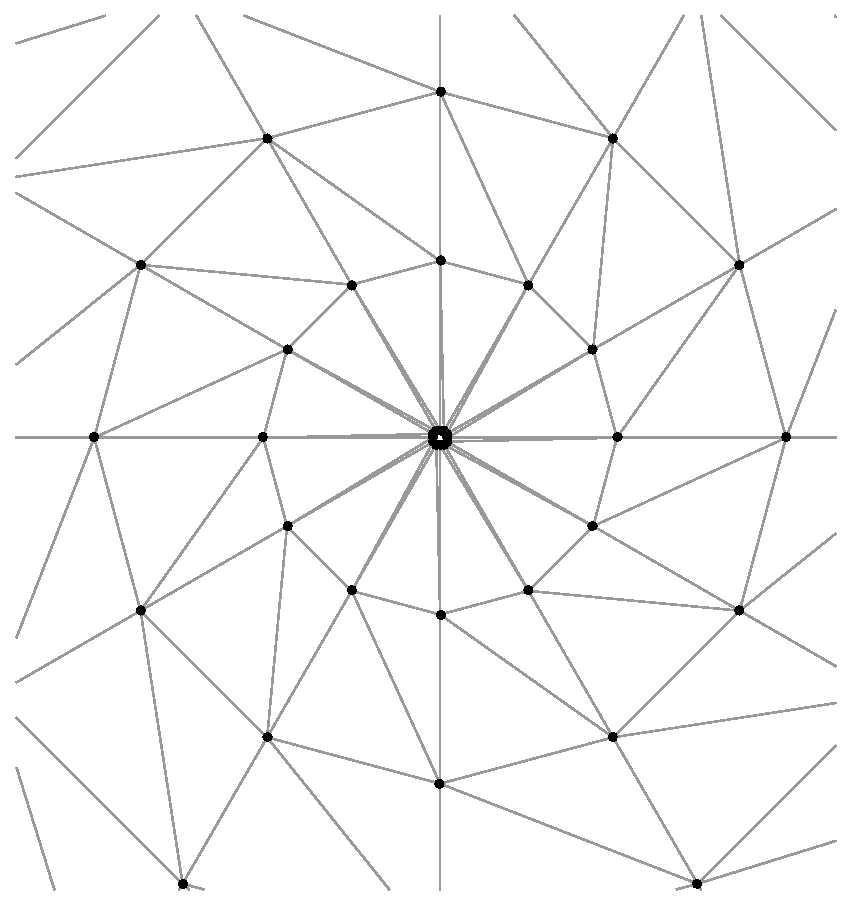
\includegraphics[width=1.0\textwidth]{figures/Comparison_smin_annulus_a.eps}
		\captionsetup{width=.4\textwidth}
		\caption{}
		\label{fig:Annulus_Plot_a}
	\end{subfigure}
	\hspace{1cm}
	\begin{subfigure}[b]{0.45\textwidth}
		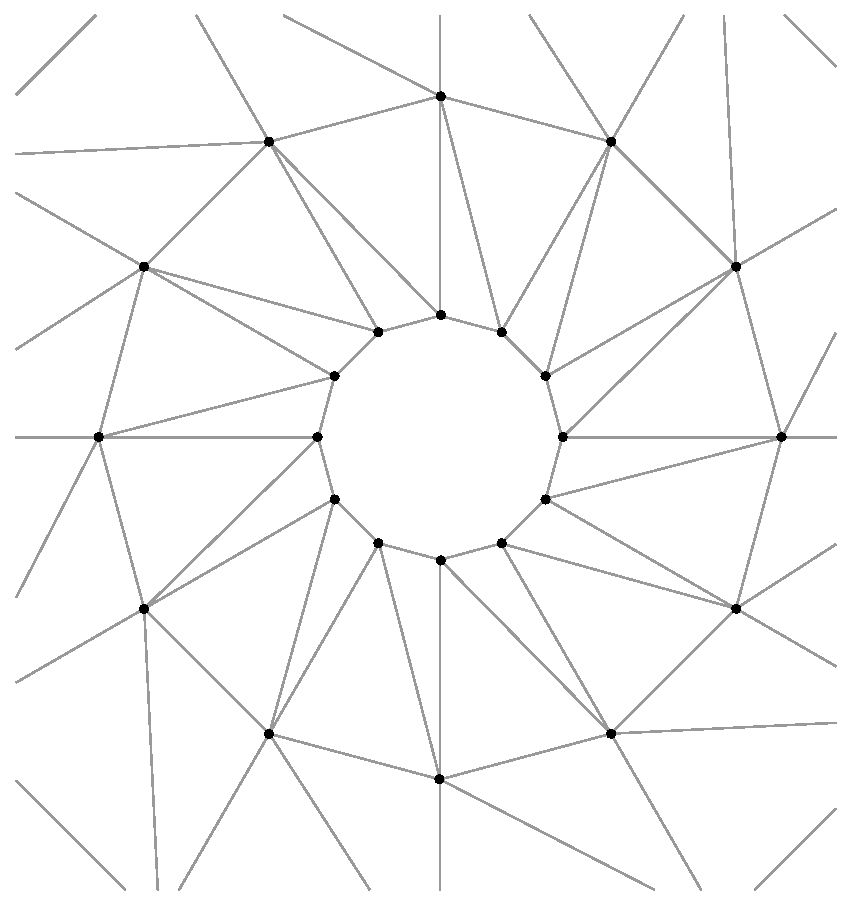
\includegraphics[width=1.0\textwidth]{figures/Comparison_smin_annulus_b.eps}
		\captionsetup{width=.4\textwidth}
		\caption{}
		\label{fig:Annulus_Plot_b}
	\end{subfigure}\hfill
		\caption{This plot presents a magnified schematic picture of the poloidal projection of the field-aligned grid center in cylindrical coordinates for two different values of \texttt{s\_min}. In plot \ref{fig:Annulus_Plot_a} a very small value for \texttt{s\_min} has been chosen, this is compared to a larger value for plot \ref{fig:Annulus_Plot_b}. It is clearly visible that the tetrahedral faces which have two corner points on the inner-most $\vartheta$-ring are only visible in \ref{fig:Annulus_Plot_b}, while they appear to be merely lines in \ref{fig:Annulus_Plot_a}.}
\label{fig:Annulus_Plot}
\end{figure}






Back to the grid generating procedure, the vector \texttt{r\_frac} is defined by
\bea*
\nonumber
\texttt{r\_frac}&=&\texttt{s\_min + [(dble(i)*(1.d0-s\_min), i=1, size(r\_frac), 1)]\&}\\
\nonumber
&&\texttt{\&/(dble(size(verts\_per\_ring))}~,
\eea
where ``\texttt{\&}'' denotes the line concatenation operator in Fortran.
Next in \texttt{create\_points\_2d}, two nested loops are implemented, the outer one iterates over the individual $\vartheta$-rings with loop index \texttt{isurf} ranging from \texttt{isurf=0} (for the center point/ring) up to \texttt{isurf=size(verts\_per\_ring)}, this loop represents the iteration over the individual $\vartheta$-rings, on which the points will lie. The inner loop iterates with index \texttt{j} ranging from \texttt{j=1} up to \texttt{verts\_per\_ring(isurf)}, this second loop represents the iteration over the individual vertices of the current $\vartheta$-ring. 
For each iteration of the outer loop, an additional vector \texttt{theta\_frac} is generated according to
\be*
\nonumber
\texttt{theta\_frac}=\texttt{[(i, i=0, n\_theta\_current-1,1)] / dfloat(n\_theta\_current)}~.
\ee
Additionally, a counter \texttt{point\_idx} is introduced, that is incremented by 1 each time a vertex is generated, this counter determines the indices of the vertices, by which their coordinates will later be accessed for the read-out of field data. The actual grid points are then generated within the loop by the code fragment
\begin{align*}
&\texttt{s} = \texttt{r\_scaling\_func(r\_frac(isurf))}\\
&\texttt{theta} = \texttt{2.d0*pi*theta\_scaling\_func(theta\_frac(j))}\\
&\texttt{verts\_sthetaphi(:,point\_idx)}=\texttt{[s,theta,0.d0]}\\
&\texttt{call magdata\_in\_symfluxcoord\_ext(1,s,psi,theta,q,dq\_ds,sqrtg,\&}\\
&\hspace{1.1cm}\texttt{\&bmod,dbmod\_dtheta,R,dR\_ds,dR\_dtheta,Z,dZ\_ds,dZ\_dtheta)}\\
&\texttt{verts\_rphiz(:,point\_idx)}=\texttt{[R,0.d0,Z]}\\
&\texttt{point\_idx = point\_idx +1}~.
\end{align*}
For scaling functions \texttt{r\_scaling\_func(x) = theta\_scaling\_func(x) = x}, equidistant grid vertices lying on the $\varphi = 0$ plane are hereby generated in symmetry flux coordinates. 
There is one optional but relevant modification that should further be discussed. Instead of generating vertices according to a distribution defined for the poloidal symmetry flux angle $\vartheta$, one can also distribute vertices according to the geometric poloidal angle $\theta$ in cylindrical coordinates. This is particularly interesting if the field aligned grid is intended to be used with the cylindrical coordinate system, as vertices distributed in $\vartheta$ experience a strong poloidal shift towards the \textit{X}-point the closer they lie to the separatrix, in fact if the outermost points were actually to lie precisely on the separatrix, they would all lie exactly at the \textit{X}-point in real space. Consequently for the grid, if the geometric $\theta$-distribution of vertices changes too drastically from one flux surface to the next, it is possible that scalar products for at least one pair of normal vectors of the individual tetrahedral planes for a given tetrahedron no longer yields a negative value (if one wants to imagine what happens here, assume a tetrahedron and drag one of the vertices through the opposing plane spanned up by the remaining three vertices, the resulting tetrahedron is literally turned inside out, this occurs as the outermost point is increasingly shifted poloidally towards the \textit{X}-point). A negative scalar product of such planes would imply that in fact the implemented logical association of vertices is invalid and the generated tetrahedron is therefore incompatible with the \textit{GORILLA} integration scheme. Thus, an interpolation routine was implemented, which transforms defined geometric angles $\theta$ back to the corresponding symmetry flux angles $\vartheta$ for a given value of $s$. The conversion subroutine is hereby called by
\begin{align*}
&\texttt{call theta\_geom2theta\_flux(s,2.d0*pi*theta\_scaling\_func(theta\_frac(j))\&}\\
&\hspace{1.1cm}\texttt{\&,theta) !optional}~,
\end{align*}
instead of directly defining \texttt{theta} in the second line of the code where the vertices are calculated. The variable that acts as a switch is denoted \texttt{geom\_flux}, where an integer value of 1 distributes the points directly in symmetry flux angle $\vartheta$ and an integer value of 2 distributes the points in geometric angle $\theta$ using the subroutine \texttt{theta\_geom2theta\_flux}.
The vertices generated by the subroutine \texttt{create\_points\_2d} are presented in figure \ref{fig:grid_theta_flux_geom}, once with vertices poloidally equidistant in symmetry flux coordinate angle $\vartheta$ (\ref{fig:grid_theta_flux}) and once with vertices poloidally equidistant in geometric angle $\theta$ (\ref{fig:grid_theta_geom}). The grey lines indicate how these points will be connected in cylindrical coordinates to form the tetrahedral mesh, mind that tetrahedra are here represented by triangles in the poloidal projection. On the left side, it can be seen that in figure \ref{fig:grid_theta_flux} some lines close to the separatrix do indeed intersect, this leads to a corrupted mesh logics in cylindrical coordinates that causes errors with the \textit{GORILLA} integrator, on the right side, figure \ref{fig:grid_theta_geom} does not show intersections, thus, this grid is compatible with \textit{GORILLA} for computations done in cylindrical coordinates. It should, however, be emphasized, that this problem only occurs for the field-aligned grid when changing to cylindrical coordinates, as long as calculations are performed in symmetry flux coordinates, geometrically aligned grids become in that case obsolete.
\begin{figure}[ht!]
	\begin{subfigure}[b]{0.45\textwidth}
		\centering
		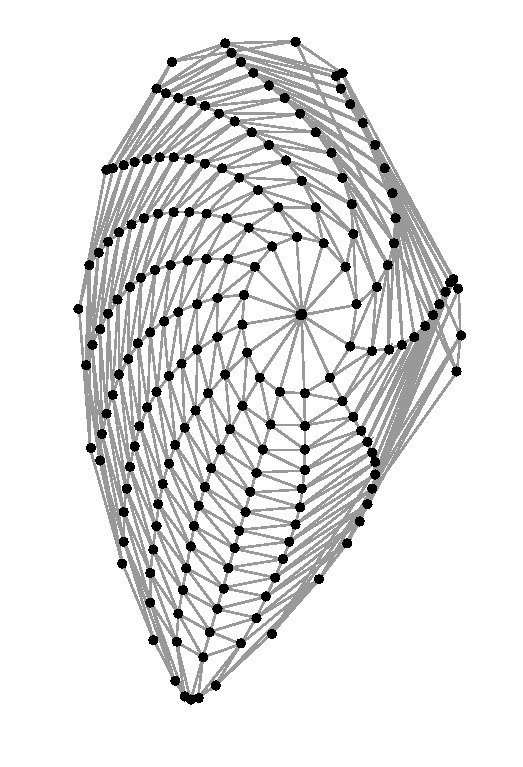
\includegraphics[width=1.0\textwidth]{figures/grid_flux_theta_meshed.eps}
		\captionsetup{width=1\textwidth}
		\caption{vertices are here poloidally equidistant in symmetry flux angle $\vartheta$}
		\label{fig:grid_theta_flux}
	\end{subfigure}
	\hfill
	\begin{subfigure}[b]{0.45\textwidth}
		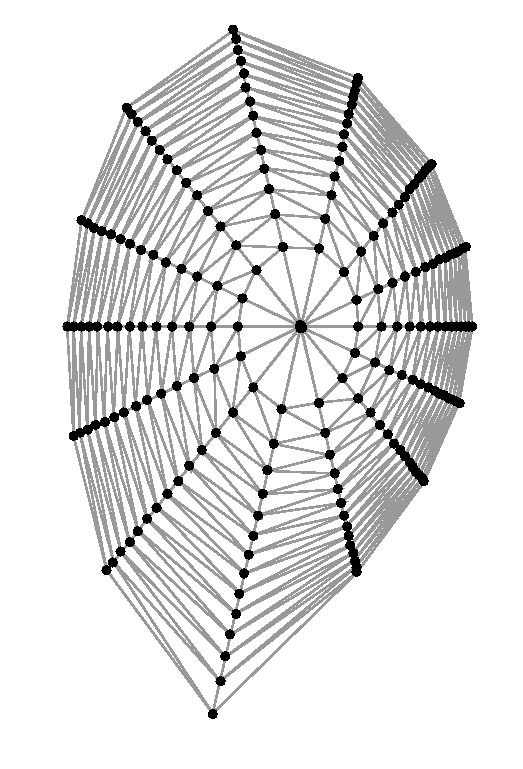
\includegraphics[width=1.0\textwidth]{figures/grid_geom_theta_meshed.eps}
		\captionsetup{width=1\textwidth}
		\caption{vertices are here poloidally equidistant in geometrical angle $\theta$}
		\label{fig:grid_theta_geom}
	\end{subfigure}\hfill
		\caption{Poloidal projection of field aligned grids in cylindrical coordinates of grid size $(N_s,N_\vartheta) = (14,14)$, vertices are indicated by black dots, the grey lines in the back indicate how these vertices will later be connected to form tetrahedra, mind that for \ref{fig:grid_theta_flux} intersections occur close to the separatrix, while for \ref{fig:grid_theta_geom} this problem was circumvented by aligning the vertices equidistantly in geometrical angle $\theta$}
\label{fig:grid_theta_flux_geom}
\end{figure}

\subsubsection{extrude\_points}
The next step in constructing the vertices for the 3D-grid in subroutine \texttt{create\_points} is now to extrude these points symmetrically into the toroidal ($\varphi$) direction. This extrusion is realized in subroutine \texttt{extrude\_points(verts\_per\_slice,nphi,phi\_position,}\\
\texttt{verts\_sthetaphi/verts\_rphiz)}, with
\begin{align*}
&\texttt{verts\_per\_slice = sum(verts\_per\_ring) + verts\_per\_ring(1)}
\end{align*}
if the boolean \texttt{repeat\_center\_point} is \texttt{true} and
\begin{align*}
&\texttt{verts\_per\_slice = sum(verts\_per\_ring) + 1}
\end{align*}
otherwise. The remaining parameters \texttt{nphi}, \texttt{phi\_position} and \texttt{verts\_sthetaphi/verts\_rphiz} represent the number of grid points in toroidal direction, the index of the toroidal component $\varphi$ in the current coordinate system (the value is hereby 2 for cylindrical coordinates $(R,\varphi,Z)$ and 3 for symmetry flux coordinates $(s,\vartheta,\varphi)$) and the coordinates of the vertices that are to be extruded, respectively. The last parameter acts here as an \texttt{inout}-variable where the first \texttt{verts\_per\_slice} number of points are the input and the remaining components are returned by the subroutine. It should furthermore be mentioned, that some liberty has been assumed in citing the fortran syntax as \texttt{verts\_sthetaphi/verts\_rphiz} means here that either one can be the input, but directly evaluating this expression would return a syntax error. Using the defined parameters, the point extrusion is performed by copying the previously computed two-dimensional vertex coordinates and saving them together with the appropriate $\varphi$-positions. This is a purely index-based operation, given by 
\begin{align*}
&    \texttt{do i = 2, nphi}\\
& \hspace{1.cm}  \texttt{vert\_idx = (i-1)*verts\_per\_slice+1}\\
& \hspace{1.cm}  \texttt{phi = (2.d0*pi/field\_periodicity*(i-1))/nphi}\\
& \hspace{1.cm}  \texttt{points(:,vert\_idx:vert\_idx+verts\_per\_slice-1) = \&}\\
& \hspace{2.cm}  \texttt{\& points(:, 1:verts\_per\_slice)}\\
& \hspace{1.cm}  \texttt{points(phi\_position,vert\_idx:vert\_idx+verts\_per\_slice-1)=phi}\\
&    \texttt{end do}
\end{align*}
where \texttt{points} is a placeholder for vertex coordinates \texttt{verts\_sthetaphi/verts\_rphiz} and \texttt{field\_periodicity} denotes the previously introduced periodicity factor of the magnetic field, this is 1 for the axisymmetric field and can have a different integer value for a stellarator configuration (e.g. field\_periodicity = 5 for a stellarator field that is invariant under a coordinate shift of magnitude $\Delta\varphi=2\pi/5$ in toroidal direction). The coordinates for all grid vertices have now been computed, the subroutine \texttt{extrude\_points} ends here.
\subsubsection{calc\_mesh}

The final step in constructing the field aligned grid is to take the generated vertices, and logically connect them to form tetrahedra in a way, that no unassigned spaces exist within the given coordinate space (the only exception here is the annulus in real space due to the degeneracy of the poloidal symmetry flux component at the magnetic axis, as discussed previously). 
This contruct will be referred to as mesh, which is calculated by the subroutine \texttt{calc\_mesh(verts\_per\_ring, nphi, verts\_rphiz(:, :nvert / nphi), ntetr, verts, neighbours, neighbour\_faces, perbou\_phi, perbou\_t}\\
\texttt{heta, repeat\_center\_point = .true.)}. This is called from the subroutine \texttt{make\_gr}\\
\texttt{id\_aligned}, as shown in figure \ref{fig:make_tetra_grid_code_structure}. Subroutine parameters, that have not yet been introduced, are \texttt{verts}, \texttt{neighbours}, \texttt{neighbour\_faces}, \texttt{perbou\_phi} and \texttt{perbou\_theta}. These variables denote placeholders for tetrahedron related data, where \texttt{verts(1:4,nte}
\texttt{tr)} stores the indices of the four corner vertices for each tetrahedron, \texttt{neighbours(1:4,}
\texttt{ntetr)} the indices of the neighboring tetrahedra ($1:\texttt{ntetr}$) which are lying adjacent to the four faces of the given tetrahedron, \texttt{neighbour\_faces(1:4,ntetr)} the face indices ($1..4$) that denote which face of the neighbor is lying adjacent to the current tetrahedron, \texttt{perbou\_phi(1:4,ntetr)} which tetrahedral faces lie on the periodic boundary in $\varphi$ direction where 0 is the default value for all tetrahedra, 1 is the value at the $\varphi = 2\pi$ boundary and -1 at the $\varphi = 0$ boundary, this is analogously implemented for \texttt{perbou\_theta} which treats the periodic boundary conditions in $\vartheta$ direction. Upon generation of the tetrahedra, these data are computed and subsequently saved in the previously introduced fortran type  \texttt{tetrahedron\_grid} given in table \ref{tab_type_tetrahedron}, there the tetrahedra are made available for further computations.

Next, the meshing algorithm will be explained in more detail. In order to be able to understand the ideas behind this algorithm, one needs to take a closer look at how the vertices are indexed. For this, a set of poloidal vertices (i.e. $\varphi=0$) is given in figure \ref{fig:verts_slices}. Here, one can see that vertices are first indexed in $\vartheta$ direction (along the $\vartheta$ rings which are horizontal sets of vertices in this represenation) where due to periodic boundary conditions in $\vartheta$ the first vertex appears twice, once for $\vartheta = 0$ and once for $\vartheta = 2\pi$. Subsequently, the vertices of the adjacing $\vartheta$ ring are indexed in the same fashion up to index \texttt{verts\_per\_slice}, which is the number of vertices on the $\varphi=0$ plane. Due to axisymmetry of the grid, the indices of the vertices that lie on the next slice (in positive $\varphi$ direction) have the exact same coordinates in the poloidal projection as the vertices lying on the first slice ($\varphi=0$), only the toroidal component differs by $\Delta\varphi = 2\pi/\texttt{nphi}$ from one slice to the next. The word \textit{slice} was chosen in this context, as it figuratively refers to a cake (the grid) being sliced into \texttt{nphi} pieces of equal size, here the vertices lie on the slice faces. In this analogy, two adjacent slice faces are created by the same cut, in the grid the cuts themselves represent the slices on which the vertices lie, whereas the cake pieces can be thought of as the space inbetween these slices which will be covered by the tetrahedra. This analogy was given to justify the selected terminology and will be no longer dwelled upon. The important information, that one can take from this picture is, however, that in the poloidal projection the vertices of different slices are equivalent and thus, the index for each vertex is incremented by \texttt{verts\_per\_slice} to obtain the index of the vertex in the next slice. To account for periodicity in $\varphi$, the resulting index is taken \texttt{modulo(index,nvert)}. The indices for the second slice are given in parentheses next to the vertex indices of the first slice in figure \ref{fig:verts_slices}.

\begin{figure}[!ht]
	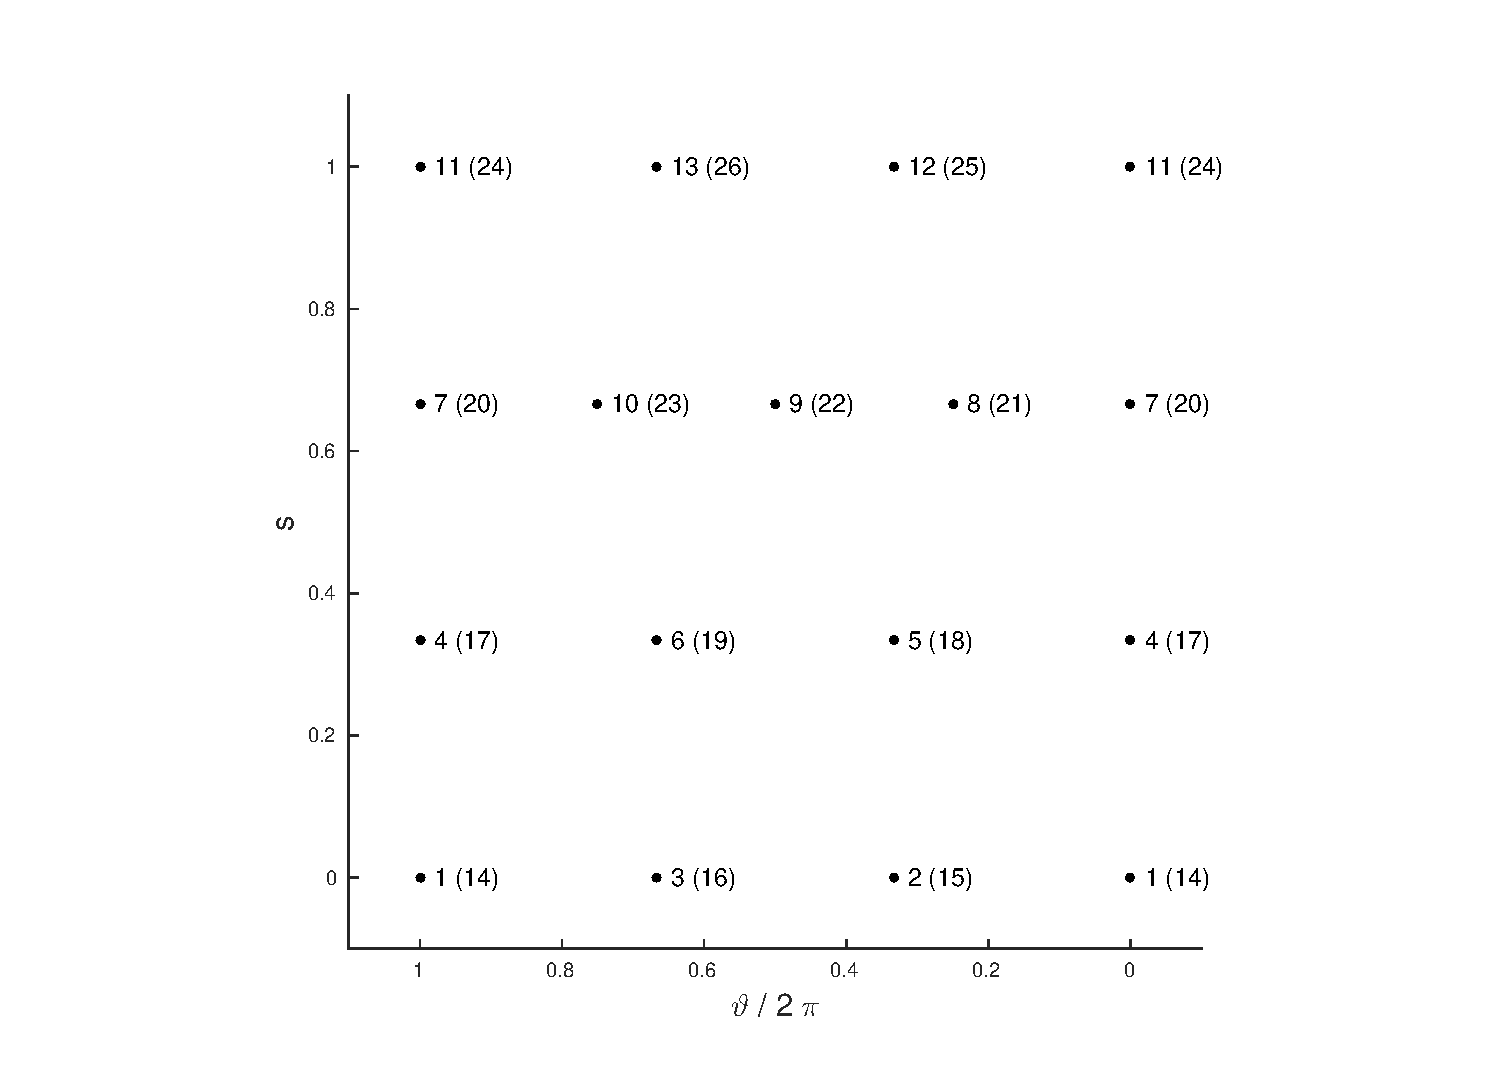
\includegraphics[width=1\textwidth]{figures/vertices_2d_slices.eps}
	\caption{Grid vertex indices  for the first $\varphi$-slice and in parentheses the indices of the next slice, the indices between slices differ by a constant value \texttt{verts\_per\_slice} which is equal to 13 for this configuration}
	\label{fig:verts_slices}
\end{figure}

For the cylindrical contour grid, the next step is to connect the vertices to form hexahedra, which are each comprised of six tetrahedra. However, this approach is not possible as it would require that each $\vartheta$ ring had the exact same number of vertices, which is generally no longer the case. Instead, prisms are used to connect the vertices, these prisms have the property that their vertices can directly be indexed to form three tetrahedra for each prism. The two types of prisms that are used to construct the grid are shown in figure \ref{fig:2prims_comp}. These prisms can be associated with certain orientations which are here denoted either \textit{top facing} or \textit{bottom facing}. This can be understood by taking a look at figure \ref{fig:verts_slices}. Here, in the lower right corner of the graph, the vertices with indices 1, 2, 4 and 5 can be connected in the poloidal plane by two triangles with the corner points for the first triangle \{1, 2, 5\} corresponding to prism vertices \{0, 2, 3\} for the top facing prism and the corner points for the second triangle \{1, 4, 5\} to prism vertices \{0, 1, 2\} for the bottom facing prism, respectively. The first triangle has one edge on the upper $\vartheta$-ring, while the second triangle has one edge on the lower $\vartheta$ ring, hence the naming top facing and bottom facing. These triangles are in fact the cross sectional representation of the prisms, which are essentially axisymmetrically extruded triangles. The use of prisms is hereby only possible due to the axisymmetric arrangement of vertices on different slices. 

\begin{figure}[!ht]
	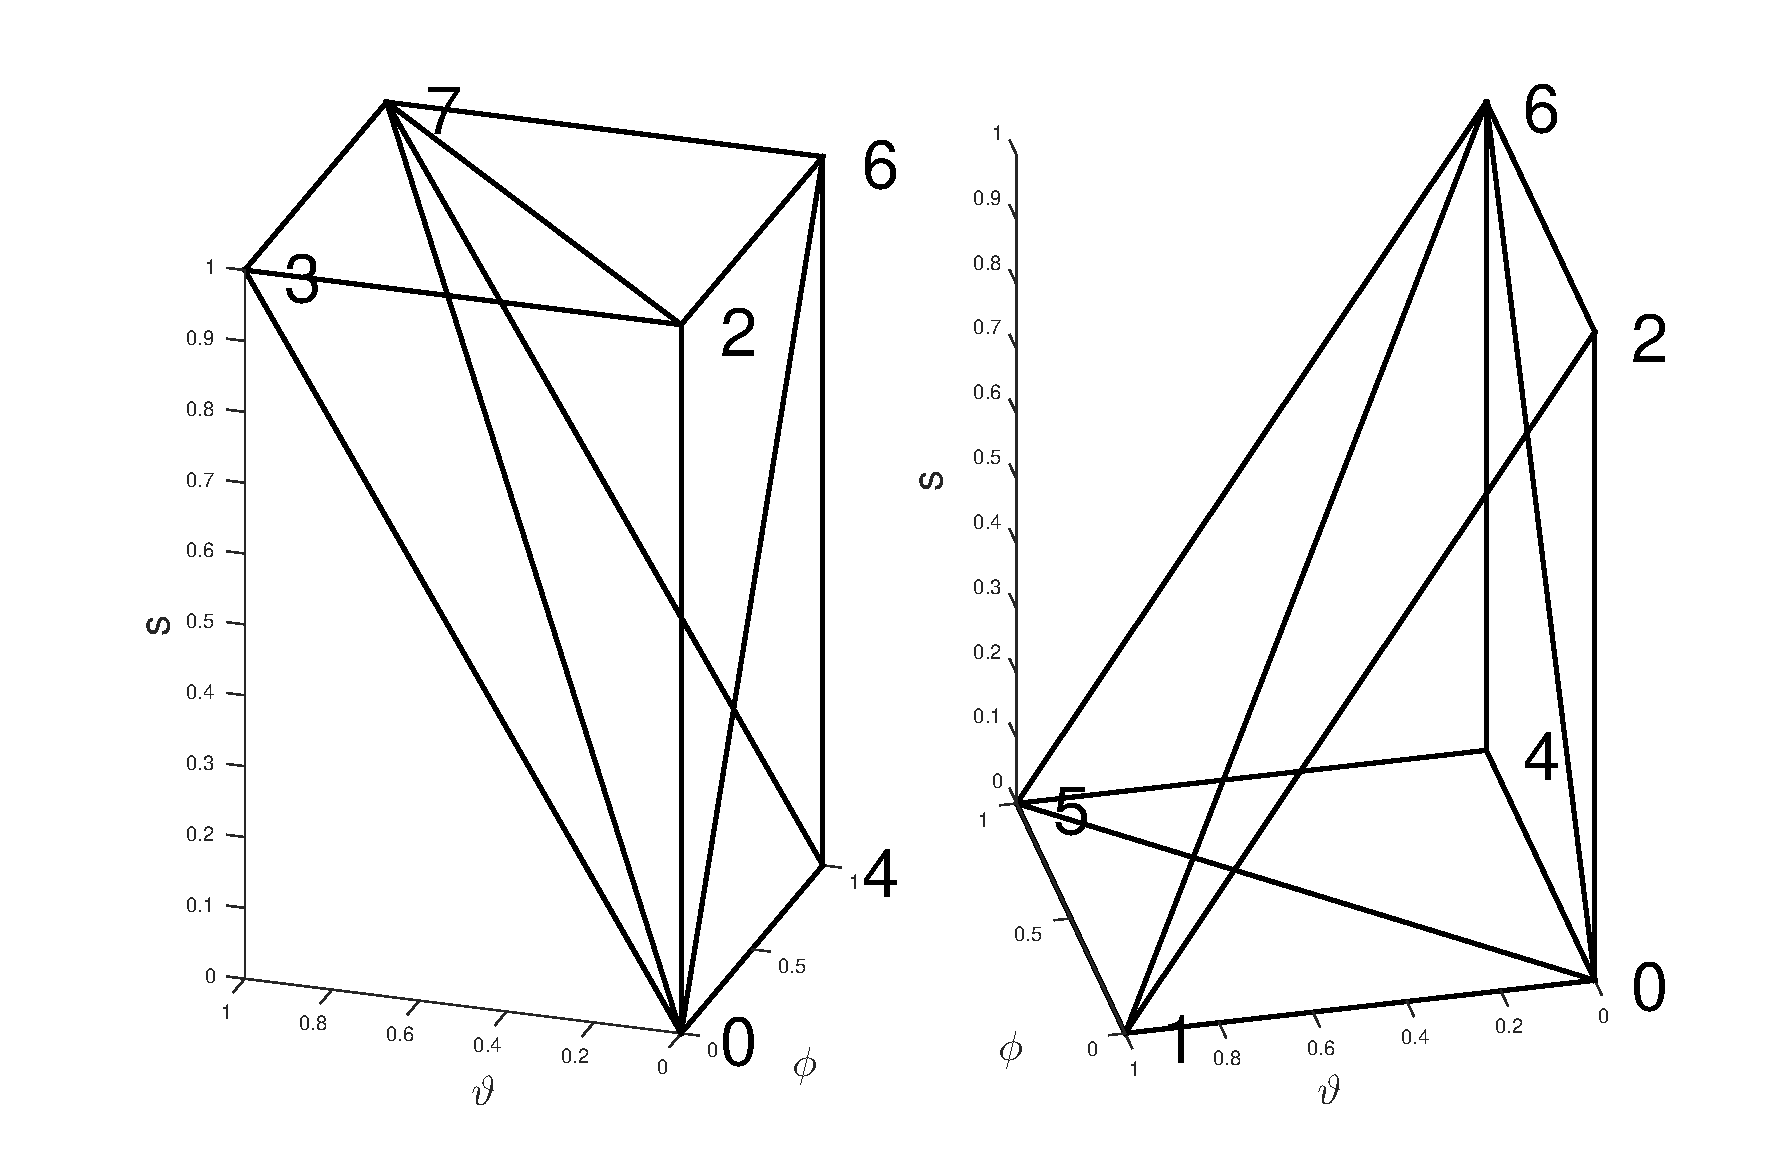
\includegraphics[width=1\textwidth]{figures/2Prisms_comparison.eps}
	\caption{Prisms used to index tetrahedra, top facing prism on the left and bottom facing prism on the right}
	\label{fig:2prims_comp}
\end{figure}
 
The approach is now to use these two types of prisms to link all vertices of the individual $\vartheta$-rings to the face vertices of the two presented prism types. By doing so, a full slice of the grid will be constructed, where each prism is subsequently split up into three tetrahedra by indexing. Additionally, the tetrahedron properties \texttt{verts}, \texttt{neighbours}, \texttt{neighbour\_faces}, \texttt{perbou\_phi} and \texttt{perbou\_theta} are computed upon generation.
It was already discussed, that the vertices in the poloidal plane can be connected by triangles representing the prisms. The question is merely, how the triangles are to be arranged, such that the poloidal projection of the grid is fully and unambiguously covered by triangles. For this, the Delaunay condition is used to determine if a proposed triangle has desirable properties, i.e. a maximal smallest interior angle. In the following, the triangles and their associated prisms will be collectively referred to as segments. 
A concrete example shall allow the reader to get a clearer image of how this process is implemented.
One is first interested to mesh the vertices of the first two $\vartheta$-rings, therefore one starts by computing how many segments can be put into this set of points. Taking poloidal periodicity into account, this is simply obtained by taking the sum of the number of vertices of the two rings. Next, one takes the first vertex of the ring (for the first ring, the first vertex has index 1) and computes the indices of the neighboring vertices \{2, 4, 5\} by adding to the current vertex index the values 1, \texttt{n\_verts\_lower} and \texttt{n\_verts\_lower}+1, respectively. For these four indices of the current vertex itself and its neighbors, the poloidal coordinate components are evaluated and saved in counter clockwise order into variables \texttt{u}, \texttt{v}, \texttt{p} and \texttt{q}. This is necessary for further evaluation of the Delaunay condition.    
The current configuration is depicted in figure \ref{fig:uvpq}.

 \begin{figure}[!ht]
 \begin{center}
	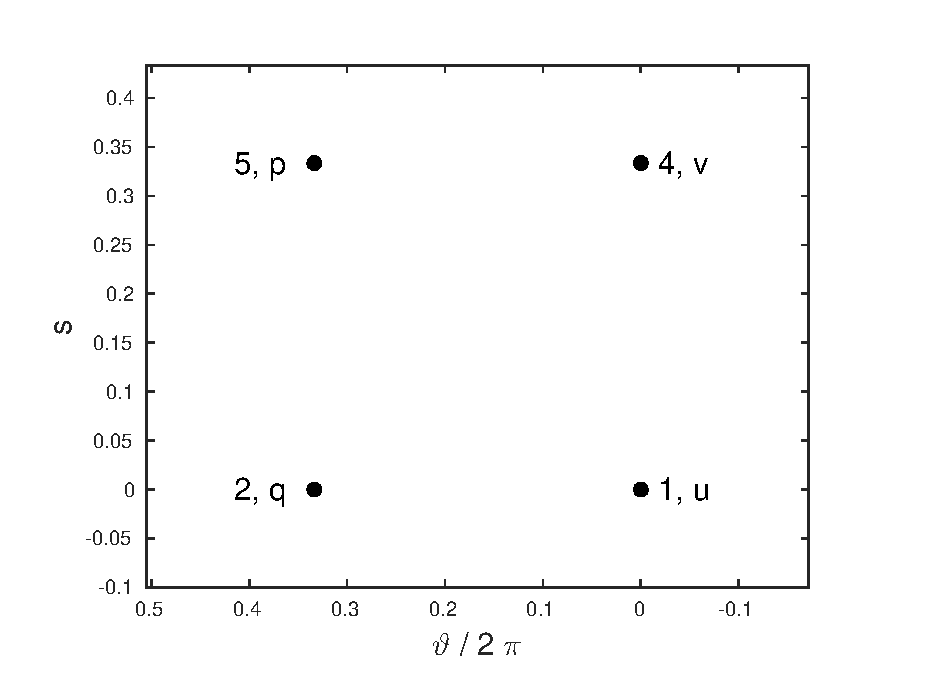
\includegraphics[width=0.5\textwidth]{figures/uvpq.eps}
	\caption{Extracted lower right corner domain of figure \ref{fig:verts_slices}, for computing the Delaunay condition for the first prism, the poloidal coordinate components of the neighboring vertices to index 1 are saved into variables \texttt{u}, \texttt{v}, \texttt{p} and \texttt{q}, whereas for this case the coordinate tuples [$\vartheta, s$] are \texttt{u = [0,0]}, \texttt{v = [0, 0.33]}, \texttt{p = [0.33,0.33]} and \texttt{q = [0.33,0]}}
	\label{fig:uvpq}
	\end{center} 
\end{figure}
Next, one must propose a segment orientation (top facing or bottom facing) and compute the Delaunay condition accordingly. By default, for each $\vartheta$-ring, the top facing orientation is initially proposed. Here, this means that the points \texttt{u}, \texttt{v} and \texttt{p} are linked to form the prism face. The Delaunay condition now states, that if one computes the circumcircle to the triangle spanned by these three points, the remaining point \texttt{q} may only lie outside this circumcircle or at most exactly on the circumcircle, in which case the Delaunay condition is ambiguous and both prism orientations are allowed.
The Delaunay condition for the top facing triangle is hereby given by \cite{Delaunay_triangulation}
 \begin{align*}
&    \texttt{a = u(1) - q(1)}\\
&    \texttt{b = u(2) - q(2)}\\
&    \texttt{c = (u(1) - q(1)) ** 2.d0 + (u(2) - q(2)) ** 2.d0}\\
&    \texttt{d = v(1) - q(1)}\\
&    \texttt{e = v(2) - q(2)}\\
&    \texttt{f = (v(1) - q(1)) ** 2.d0 + (v(2) - q(2)) ** 2.d0}\\
&    \texttt{g = p(1) - q(1)}\\
&    \texttt{h = p(2) - q(2)}\\
&    \texttt{i = (p(1) - q(1)) ** 2.d0 + (p(2) - q(2)) ** 2.d0}\\
%\end{align*}
%\begin{align*}
&    \texttt{delta = a*e*i + b*f*g + c*d*h - c*e*g - b*d*i - a*f*h}\\
&    \texttt{if (delta<=0.d0) then}\\
& \hspace{1.cm}  \texttt{delaunay\_condition = .true.}\\
&    \texttt{else}\\
& \hspace{1.cm}  \texttt{delaunay\_condition = .false.}\\
&    \texttt{endif}\\
\end{align*}
The result from this condition is, that if \texttt{delaunay\_condition =.true.} is returned, the top facing configuration is accepted, if not, the bottom facing configuration with corner points \texttt{u}, \texttt{v} and \texttt{q} is selected instead. This is valid, as this procedure corresponds to the so-called Delaunay flip, which states that if four vertices are linked to form two adjacent triangles that do not satisfy the Delaunay condition (e.g. triangles \{u, v, p\} and \{u, p, q\}), one can always obtain two triangles that do satisfy the condition by flipping the orientation of the line segment that divides the two triangles (i.e. leading to new triangles \{u, v, q\} and \{v, p, q\}) \cite{Delaunay_triangulation}.
 \begin{figure}[!ht]
 \begin{center}
	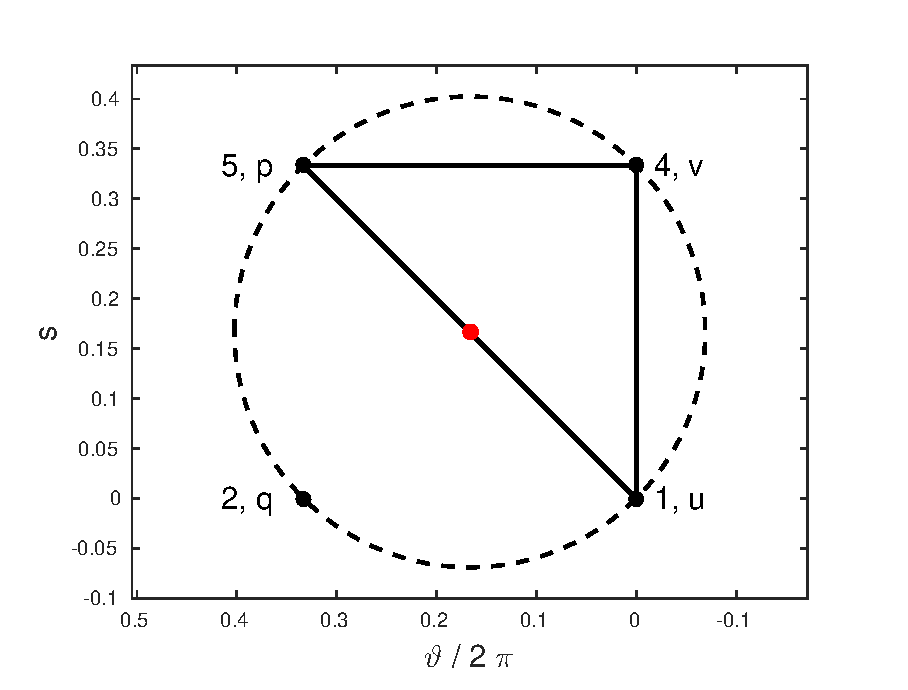
\includegraphics[width=0.5\textwidth]{figures/uvpq_Delaunay.eps}
	\caption{Visualization of the Delaunay condition for the top facing segment (solid line), if \texttt{q} lies outside or at most exactly on the circumcircle (dashed line, center marked by red dot) around \{\texttt{u}, \texttt{v}, \texttt{p}\} the Delaunay condition is satisfied. Since for the shown configuration all four vertices lie on the circumcircle the Delaunay condition is satisfied for both the top facing and bottom facing orientation, whenever this occurs the top facing orientation is assumed in this approach.}
	\label{fig:uvpq_Delaunay}
	\end{center} 
\end{figure}

Upon determining for \texttt{u}, \texttt{v}, \texttt{p} and \texttt{q} which proposed orientation is accepted, the next step is to associate the three vertices of the accepted configuration (i.e. \{u, v, p\} for top facing or \{u, v, q\} for bottom facing) with the poloidal face vertices of the prisms shown in figure \ref{fig:2prims_comp}. Here the three vertices either correspond to prism vertex indices \{0, 2, 3\} for the top facing or \{0, 1, 2\} for the bottom facing  configuration. The grid vertex indices of the remaining prism vertices are found as follows.\\
In order to explain this process, one must first take a look at the binary representation of the prism vertex indices and the corresponding normalized offsets of the vertex positions in symmetry flux space with respect to prism vertex 0 (e.g. for prism vertex 3 of the bottom facing configuration, the vertex has an offset in the $s$ and $\vartheta$ direction, but not in the $\varphi$ direction, thus the normalized offset in $(\varphi, s, \vartheta)$ is given by $(0, 1, 1)$). The binary representation of the prism vertex indices and the corresponding normalized positional offsets are given in tab. \ref{tab:binary_prisms}. 
 
\begin{centering}
	\begin{table}[H]
		\caption{Binary representation of prism vertices the corresponding normalized positional offsets}
		\begin{tabular}{|l|l|l|l|l|}
			\hline
			 \rowcolor{lightgray}
			Index&Binary&$\varphi$-offset &$s$-offset &$\vartheta$-offset \\
			\hline
			0&0 - 0 - 0&0&0&0\\ 
			\hline
			1&0 - 0 - 1&0&0&1\\ 
			\hline 
			2&0 - 1 - 0&0&1&0\\ 
			\hline
			3&0 - 1 - 1&0&1&1\\ 
			\hline
			4&1 - 0 - 0&1&0&0\\ 
			\hline
			5&1 - 0 - 1&1&0&1\\ 
			\hline
			6&1 - 1 - 0&1&1&0\\ 
			\hline
			7&1 - 1 - 1&1&1&1\\ 
			\hline
		\end{tabular}
		\label{tab:binary_prisms}	
	\end{table}
\end{centering}

One can clearly see that the bitwise representation of the prism vertices coincides with the individual normalized positional offsets in directions $\varphi$, $s$ and $\vartheta$, respectively. Thus, due to the specific way in which the vertices are arranged, the indices of the prism vertices can be directly obtained from the normalized positional offsets via

\begin{align}
    \texttt{vertex\_index} =&\texttt{base\_idx + theta\_offset + s\_offset*n\_verts\_lower\&}\label{eq:get_indices_from_offsets}\\
&\texttt{\&+ phi\_offset*verts\_per\_slice}~,\nonumber
\end{align}

where \texttt{base\_idx} denotes the index of the current grid vertex corresponding to prism index 0 and \texttt{n\_verts\_lower} is the number of poloidal grid points for the \textit{lower} (i.e. smaller $s$-component) $\vartheta$-ring. In this concrete example for the first grid segment, \texttt{base\_idx} is equal to 1. 
Using \ref{eq:get_indices_from_offsets}, the remaining grid vertex indices for the corresponding prism vertices are obtained to fully define the prism in the symmetry flux coordinate space. Next, tetrahedra are constructed using grid vertex indices for the corresponding prism vertices. The way that the prism vertices are combined to form tetrahedra can be deduced from figure \ref{fig:2prims_comp}, for simplicity the tetrahedron vertex indices are also given in table \ref{tab:tetrahedron_indices_for_prisms}.

\begin{centering}
	\begin{table}[H]
		\caption{List of tetrahedron types with corresponding prism vertex indices for both top and bottom facing prism orientations}
		\begin{tabular}{|l|l|l|}
			\hline
			 \rowcolor{lightgray}
			Tetrahedron type&Prism vertex indices&Prism orientation\\
			\hline
			1&0, 2, 3, 7&top facing\\			
			\hline
			2&0, 2, 6, 7&top facing\\		
			\hline
			3&0, 4, 6, 7&top facing\\			
			\hline
			4&0, 1, 2, 6&bottom facing\\			
			\hline
			5&0, 1, 5, 6&bottom facing\\			
			\hline
			6&0, 4, 5, 6&bottom facing\\			
			\hline
		\end{tabular}
		\label{tab:tetrahedron_indices_for_prisms}	
	\end{table}
\end{centering}

Since now the indices of the tetrahedron vertices are known for the first three tetrahedra, their values are saved into the first three rows of \texttt{verts}. Quantities that remain unknown are \texttt{neighbours}, \texttt{neighbour\_faces}, \texttt{perbou\_phi} and \texttt{perbou\_theta}. Next, one is interested in computing the \texttt{neighbours} with the associated \texttt{neighbour\_faces} for the tetrahedra that belong to a given segment. For this, it must first be understood what types of neighbors exist for such a segment, for this it is helpful to take another look at figure \ref{fig:2prims_comp}. Here, one can see that there exist different tetrahedron boundaries on the inside of the segments as well as boundaries on the outside of the segment. More precisely, for three tetrahedra with four faces each, there exist 12 tetrahedral boundaries for any given segment. For instance for the top facing prism, there are four interior boundaries in the segment (internal boundaries are double-counted as they belong to two tetrahedra each), furthermore the segment has two boundaries pointing in the $\varphi$ direction (with one pointing in $(+\varphi)$-direction and one pointing in $(-\varphi)$-direction), two more boundaries point in the ($+s$)-direction, the remaining four boundaries point to the neighboring tetrahedra on the same $\vartheta$-ring, with two boundaries on the ($+\vartheta$) side of the prism and the last two on the ($-\vartheta$) side. For the bottom facing segment, this is analogous with the difference, that two boundaries now point in the $(-s)$-direction instead of the  $(+s)$-direction. Moreover, to recapitulate, the definition of a neighbor with index $i$ (1:4) to a given tetrahedron is the index of the tetrahedron that shares the three vertices that lie on the plane, spanned by the current tetrahedron vertices excluding the $i^{th}$ vertex. For example, the third face of a tetrahedron lies on the plane spanned by tetrahedron vertices \{1, 2, 4\}, if this tetrahedron is for instance of type 1 the prism indices for this face would be \{0, 2, 7\} and the grid vertex indices would be elements \{1, 2, 4\} of the corresponding row in \texttt{verts}. The quantity \texttt{neighbour\_faces(i)} with value $j$ (1..4) is defined as the index of the face through which one enters the neighboring tetrahedron at face $i$ (1..4). For example, given two tetrahedra with indices \texttt{ind\_1} and \texttt{ind\_2} that share a common plane on vertices \{2, 3, 4\} in the system of the first tetrahedron and vertices \{1, 2, 3\} for the second tetrahedron, the second tetrahedron is the first neighbor with respect to the first one, thus \texttt{neighbours(ind\_1,1)=ind\_2}. Furthermore one enters the second tetrahedron through its fourth plane, thus \texttt{neighbour\_faces(ind\_1,1)=4} for the first tetrahedron. Conversely, when starting from the second tetrahedron, the first tetrahedron is now the fourth neighbor and one enters the tetrahedron through the first face, therefore \texttt{neighbours(ind\_2,4)=ind\_1} and \texttt{neighbour\_faces(ind\_1,4)=1}.
Generally, for any tetrahedron \texttt{neighbours(neighbours(ind\_1,i),neighbour\_faces(ind\_1,i)) = ind\_1} must hold for all \texttt{i} if there exists an adjacent tetrahedron at face \texttt{i}.
A summary of all tetrahedral boundaries is given in table \ref{tab:tetrahedron_boundaries}. Using this information, one can find the internal neighbors within the segment, furthermore, one can directly compute the indices of the neighbors in $\varphi$ direction due to the axisymmetric configuration of the system. Here, one should only keep in mind, that when shifting the index of the current tetrahedron by the relative neighbor index of table \ref{tab:tetrahedron_boundaries}, one must account for index periodicity in $\varphi$ by subsequently shifting the resulting index into the valid regime of tetrahedron indices [1, \texttt{ntetr}], where \texttt{ntetr} denotes the total number of tetrahedra. Indices can hereby be shifted into this regime using the modulo function in
\[\texttt{index\_shifted = modulo(index-1,ntetr)+1}~.\]     

\begin{centering}
	\begin{table}[H]
		\caption{This table shows a summary of all possible types of tetrahedron boundaries and if possible, the relative indices for the neighboring tetrahedron at this boundary with respect to the current tetrahedron index (however, not accounting for toroidal periodicity here, thus, indices must still be shifted into the valid domain [1,\texttt{ntetr}] using the modulo function). If a neighboring tetrahedron can be directly specified, also the index of the adjacent face of the neighbor is given. Question marks denote quantities that depend on how the grid is meshed and which are thus not yet specified at the point of tetrahedron creation.}
		\begin{tabular}{|l|l|l|l|l|l|}
\hline
			 \rowcolor{lightgray}
			Tetrahedron&Face&Vertices&Boundary&Relative neighb. index&n. Face\\
\hline	
			%Tetrahedron 				%Face	%Vertices			%Boundary		%relative neighbor	%neighbour_face		
			\textbf{1}					&1		&\{2, 3, 7\}		&$+s$			&?			&?		\\
			Type: top facing			&2		&\{0, 3, 7\}		&$+\vartheta$	&?			&?		\\
			Vertices: 	&3		&\{0, 2, 7\}		&internal		&+1			&3		\\
			\{0, 2, 3, 7\}							&4		&\{0, 2, 3\}		&$-\varphi$		&-\texttt{tetras\_per\_slice}$+2$	&1\\
\hline
			\textbf{2}					&1		&\{2, 6, 7\}		&$+s$			&?			&?		\\
			Type: top facing			&2		&\{0, 6, 7\}		&internal		&+1			&2		\\
			Vertices: 	&3		&\{0, 2, 7\}		&internal		&-1			&3		\\
			\{0, 2, 6, 7\}							&4		&\{0, 2, 6\}		&$-\vartheta$	&?			&?		\\
\hline
			\textbf{3}					&1		&\{4, 6, 7\}		&$+\varphi$		&+\texttt{tetras\_per\_slice}$-2$	&4\\
			Type: top facing			&2		&\{0, 6, 7\}		&internal		&-1			&2		\\
			Vertices: 	&3		&\{0, 4, 7\}		&$+\vartheta$	&?			&?		\\
			\{0, 4, 6, 7\}							&4		&\{0, 4, 6\}		&$-\vartheta$	&?			&?		\\
\hline
			\textbf{4}					&1		&\{1, 2, 6\}		&$+\vartheta$	&?			&?		\\
			Type: bot. facing			&2		&\{0, 2, 6\}		&$-\vartheta$	&?			&?		\\
			Vertices: 	&3		&\{0, 1, 6\}		&internal		&+1			&3		\\
			\{0, 1, 2, 6\}							&4		&\{0, 1, 2\}		&$-\varphi$		&-\texttt{tetras\_per\_slice}$+2$	&?\\
\hline
			\textbf{5}					&1		&\{1, 5, 6\}		&$+\vartheta$	&?			&?		\\
			Type: bot. facing			&2		&\{0, 5, 6\}		&internal		&+1			&2		\\
			Vertices: 	&3		&\{0, 1, 6\}		&internal		&-1			&3		\\
			\{0, 1, 5, 6\}							&4		&\{0, 1, 5\}		&$-s$			&?			&?		\\
\hline
			\textbf{6}					&1		&\{4, 5, 6\}		&$+\varphi$		&+\texttt{tetras\_per\_slice}$-2$	&?\\
			Type: bot. facing			&2		&\{0, 5, 6\}		&internal		&-1			&2		\\
			Vertices: 	&3		&\{0, 4, 6\}		&$-\vartheta$	&?			&?		\\
			\{0, 4, 5, 6\}							&4		&\{0, 4, 5\}		&$-s$			&?			&?		\\
\hline
			%\multirow{4}{0pt}\newline
		\end{tabular}
		\label{tab:tetrahedron_boundaries}	
	\end{table}
\end{centering}

So far, a single segment has been created and split into tetrahedra. The corresponding tetrahedron vertices have been saved into the first three rows of \texttt{verts}. Furthermore, the neighbor indices for the internal tetrahedron boundaries of the segment as well as the neighbors in $\varphi$-direction have been identified together with the associated adjacent faces of the neighbors. 
These values are now saved into the corresponding fields of arrays \texttt{neighbours} and \texttt{neighbour\_faces}, here it should be further noted that this array is first initialized with values $-1$ for all elements, this value indicates that no neighbor exists at the specified boundary and the domain of the grid ends. By overwriting the corresponding elements with their actual values, the tetrahedra are linked. Once this process is completed for all tetrahedra, the remaining elements which contain the value $-1$ correspond to the actual domain boundaries at $s = \texttt{s\_min}$ and $s = 1$. 

At this point of the code, however, there are still some remaining neighbors and neighboring faces for the current segment that cannot yet be computed as their values depend on how the other segments are oriented (which is again determined by the Delaunay condition). Therefore, two nested loops are implemented to construct all segments of the first $\varphi$-slice where the inner loop iterates over all segments of the current $\vartheta$-ring and the outer loop iterates over all $\vartheta$-rings. Within these loops, the approach of constructing the tetrahedra corresponds exactly to the example of the first three tetrahedra, as discussed above. After a segment is completed in the $\vartheta$-ring, depending on its orientation, either the indices for \{v, p\} (if top facing) or for \{u, q\} (if bottom facing) need to be shifted by one (i.e. in $+\vartheta$-direction) in order to obtain the new point configuration to evaluate the Delaunay condition for the next segment, this is realized via integer offsets \texttt{upper\_off} and \texttt{lower\_off}. Due to poloidal periodicity, the indices for \{u, v, p, q\} must be taken as \texttt{modulo(index-1, verts\_per\_ring\_upper)} and \texttt{modulo(index-1, verts\_per\_ring\_lower)} for \textit{upper} vertices \{v, p\} and \textit{lower} vertices \{u, q\}, respectively. This ensures that the last vertices of the current ring are correctly linked with the first vertices. Due to toroidal symmetry the remaining tetrahedra of the full grid can actually be easily obtained upon finishing the first slice by subsequently shifting the tetrahedra vertices by the number of points per slice as well as shifting the neighbor indices by the number of tetrahedra per slice. 
For a better overview, the whole procedure of the tetrahedron generation is given as pseudo-code.

\begin{align*}
&\texttt{do ring=1,n\_rings}\nonumber\\
&\hspace{1cm} \texttt{set index offsets for u, v, p, q to zero}\nonumber\\
&\hspace{1cm} \texttt{set reference point (index for first u) index to 1}\nonumber\\
&\hspace{1cm} \texttt{set prism index to 1}\nonumber\\
\end{align*}
\begin{align*}
&\hspace{1cm} \texttt{do segment=1,prisms\_per\_ring(ring)}\nonumber\\
&\hspace{2cm} \texttt{compute u, v, p, q from reference point and offsets}\nonumber\\
&\hspace{2cm} \texttt{evaluate Delaunay\_condition(u, v, p, q) for top facing prism}\nonumber\\
&\hspace{2cm} \texttt{if (Delaunay\_condition==.true.) then}\nonumber\\
&\hspace{3cm} \texttt{make top facing prism from normalized positional \&}\nonumber\\
&\hspace{4cm} \texttt{\& offsets}\nonumber\\
&\hspace{3cm} \texttt{save current prism index in top\_facing\_prisms for \&}\nonumber\\
&\hspace{4cm} \texttt{\& neighbor indexing with next ring}\nonumber\\
&\hspace{3cm} \texttt{index tetrahedra from top facing prism}\nonumber\\
&\hspace{3cm} \texttt{increment index offset for upper vertices v, p}\nonumber\\
&\hspace{2cm} \texttt{else}\nonumber\\
&\hspace{3cm} \texttt{make bottom facing prism from normalized positional \&}\nonumber\\
&\hspace{4cm} \texttt{\& offsets}\nonumber\\
&\hspace{3cm} \texttt{index tetrahedra from bottom facing prism}\nonumber\\
&\hspace{3cm} \texttt{if (.not. ring == 1) then}\nonumber\\
&\hspace{4cm} \texttt{find neighbors with corresponding prism \&}\nonumber\\
&\hspace{5cm} \texttt{\& in top\_facing\_prisms}\nonumber\\
&\hspace{3cm} \texttt{endif}\nonumber\\
&\hspace{3cm} \texttt{increment index offset for lower vertices u, q}\nonumber\\
&\hspace{2cm} \texttt{endif}\nonumber\\
&\hspace{2cm} \texttt{find internal neighbors}\nonumber\\
&\hspace{2cm} \texttt{find neighbors to adjacent phi slices}\nonumber\\
&\hspace{2cm} \texttt{if (segment ==1) then}\nonumber\\
&\hspace{3cm} \texttt{find periodic boundary faces in -theta direction}\nonumber\\
&\hspace{2cm} \texttt{endif}\nonumber\\
&\hspace{2cm} \texttt{if (.not. segment ==1 ) then}\nonumber\\
&\hspace{3cm} \texttt{find neighbors with the previous segment}\nonumber\\
&\hspace{2cm} \texttt{endif}\nonumber\\
&\hspace{2cm} \texttt{if (segment == prisms\_per\_ring(ring)) then}\nonumber\\
&\hspace{3cm} \texttt{find periodic boundary faces in +theta direction}\nonumber\\
&\hspace{2cm} \texttt{endif}\nonumber\\
&\hspace{1cm} \texttt{enddo}\nonumber\\
\end{align*}
\begin{align*}
&\hspace{1cm} \texttt{find neighbors between first and last segment in ring}\nonumber\\
&\hspace{1cm} \texttt{shift reference point to next ring by incrementing the index \&}\nonumber\\
&\hspace{2cm} \texttt{\& by n\_verts\_lower}\nonumber\\
&\hspace{1cm} \texttt{save tetrahedron quantities based on \&}\nonumber\\
&\hspace{2cm} \texttt{\& ind\_tetra(i) = (prism index-1)*3+i for i = [1..3] \&}\nonumber\\
&\hspace{2cm} \texttt{\& and increment prism index by 1}\nonumber\\
&\texttt{enddo}\nonumber\\
&\texttt{shift tetrahedra indices to obtain tetrahedra of all remaining slices}\nonumber\\
&\texttt{find periodic boundary faces in phi direction}\nonumber\\
\end{align*}
There are two code elements that were not explained yet, the first being how unknown neighbors between two adjacent prisms are found and the second being how the periodic boundaries are determined.
The first code element is implemented in subroutine \texttt{connect\_prisms}. This subroutine takes arguments \texttt{(prism\_1\_idx, prism\_2\_idx, verts, neighbours, neighbour\_faces)}, where the first three arguments are input quantities that define which adjacent prisms are being linked as well as the information which vertices these prisms contain. The latter two arguments are the two-dimensional arrays where the found neigbor properties are saved in the corresponding fields, these are, thus, inout quantities.
The approach in this subroutine is in fact very simple, one constructs two nested loops where each loop iterates over the individual tetrahedra of one of the prisms. Within these loops the vertex indices of the two tetrahedra are compared, if three vertices coincide a neighbor has been found. In such a case one has to further find for both tetrahedra which point is not contained in the other tetrahedron. Here, the position of the index in the four element vertex array of the tetrahedron which is not included in the other tetrahedron directly corresponds to the value of \texttt{neighbour\_faces} of the adjacent tetrahedron. Once a neighbor and its corresponding neighbor face have been found, the values are saved accordingly. At the end of iteration, all neighbors of the two input prisms are successfully linked, if the two prisms are indeed adjacent.\\
For the second code element, the periodicity boundaries need to be treated separately for $\vartheta$ and $\varphi$, whereas both are identically initialized with the value 0 for all elements. In the $\vartheta$-direction, depending on the orientation, the prisms at the poloidal boundary can be directly indexed according to the results of \ref{tab:tetrahedron_boundaries}. If for instance a top facing prism is the first segment in a ring, the boundaries in $-\vartheta$-direction are given by the fourth face of the second tetrahedron and the fourth face of the third tetrahedron inside the prism, respectively. Thus, the value for the periodic boundary is then saved as \texttt{theta\_perbou(ind\_tetr,i)=-1}, where \texttt{ind\_tetr} denotes the tetrahedron index and \texttt{i} the index of the face adjacent to the boundary. This is analogous for the $\vartheta=2\pi$-boundary with the differences that here the neighbors in positive $\vartheta$-direction are considered and a value of 1 is assumed in \texttt{theta\_perbou}. For the $\varphi$-direction, however, the process is in fact much simpler as it can be directly solved via indexing as both prism types have their first tetrahedron with its fourth face adjacent to the $-\varphi$ boundary and their third tetrahedron with its first face adjacent to the $+\varphi$ boundary. Thus, one can directly write
\begin{align*}
&\texttt{perbou\_phi = 0}\nonumber\\
&\texttt{perbou\_phi(4, :tetras\_per\_slice:3) = -1}\nonumber\\
&\texttt{perbou\_phi(1, n\_tetras - tetras\_per\_slice + 3::3) = 1}\nonumber\\
\end{align*}
Now, all necessary tetrahedron quantities have been successfully computed and returned to the overlying subroutine \texttt{make\_grid\_aligned}. The last step is to allocate the tetrahedra according to the type \texttt{tetrahedron \_grid} and set the necessary quantities by.

\begin{align*}
&\texttt{allocate(tetra\_grid(1:ntetr))}\nonumber\\
&\texttt{do i=1,ntetr}\nonumber\\
&\hspace{1cm}\texttt{tetra\_grid(i)\%ind\_knot = verts(:, i)}\nonumber\\
&\hspace{1cm}\texttt{tetra\_grid(i)\%neighbour\_tetr = neighbours(:, i)}\nonumber\\
&\hspace{1cm}\texttt{tetra\_grid(i)\%neighbour\_face = neighbour\_faces(:, i)}\nonumber\\
&\hspace{1cm}\texttt{tetra\_grid(i)\%neighbour\_perbou\_phi(:) = perbou\_phi(:, i)}\nonumber\\
&\hspace{1cm}\texttt{tetra\_grid(i)\%neighbour\_perbou\_theta(:) = perbou\_theta(:, i)}\nonumber\\
&\texttt{enddo}\nonumber\\
\end{align*}

The field aligned grid is now finished. In order to visualize the resulting grid, some figures are shown below.
\newpage
\begin{figure}[!ht]
	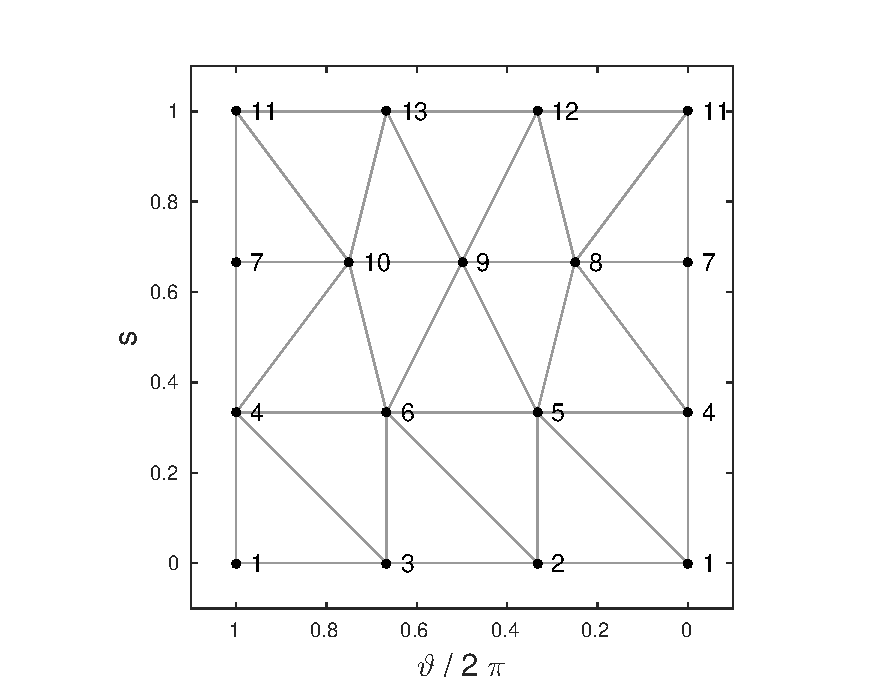
\includegraphics[width=1\textwidth]{figures/Delaunay_Connected_PrismFaces.eps}
	\caption{Depiction of the field aligned grid in symmetry flux coordinates with an increased number of poloidal vertices at $s=2/3$, vertex coordinates were extended poloidally to 2$\pi$ to make the representation cleaner}
	\label{fig:Delaunay_Connected_Faces}
\end{figure}

One can see in figure \ref{fig:Delaunay_Connected_Faces}, that even though a variable number of vertices was used for the different $\vartheta$-rings, the algorithm produces a very well aligned grid using the Delaunay condition.

\begin{figure}[!ht]
	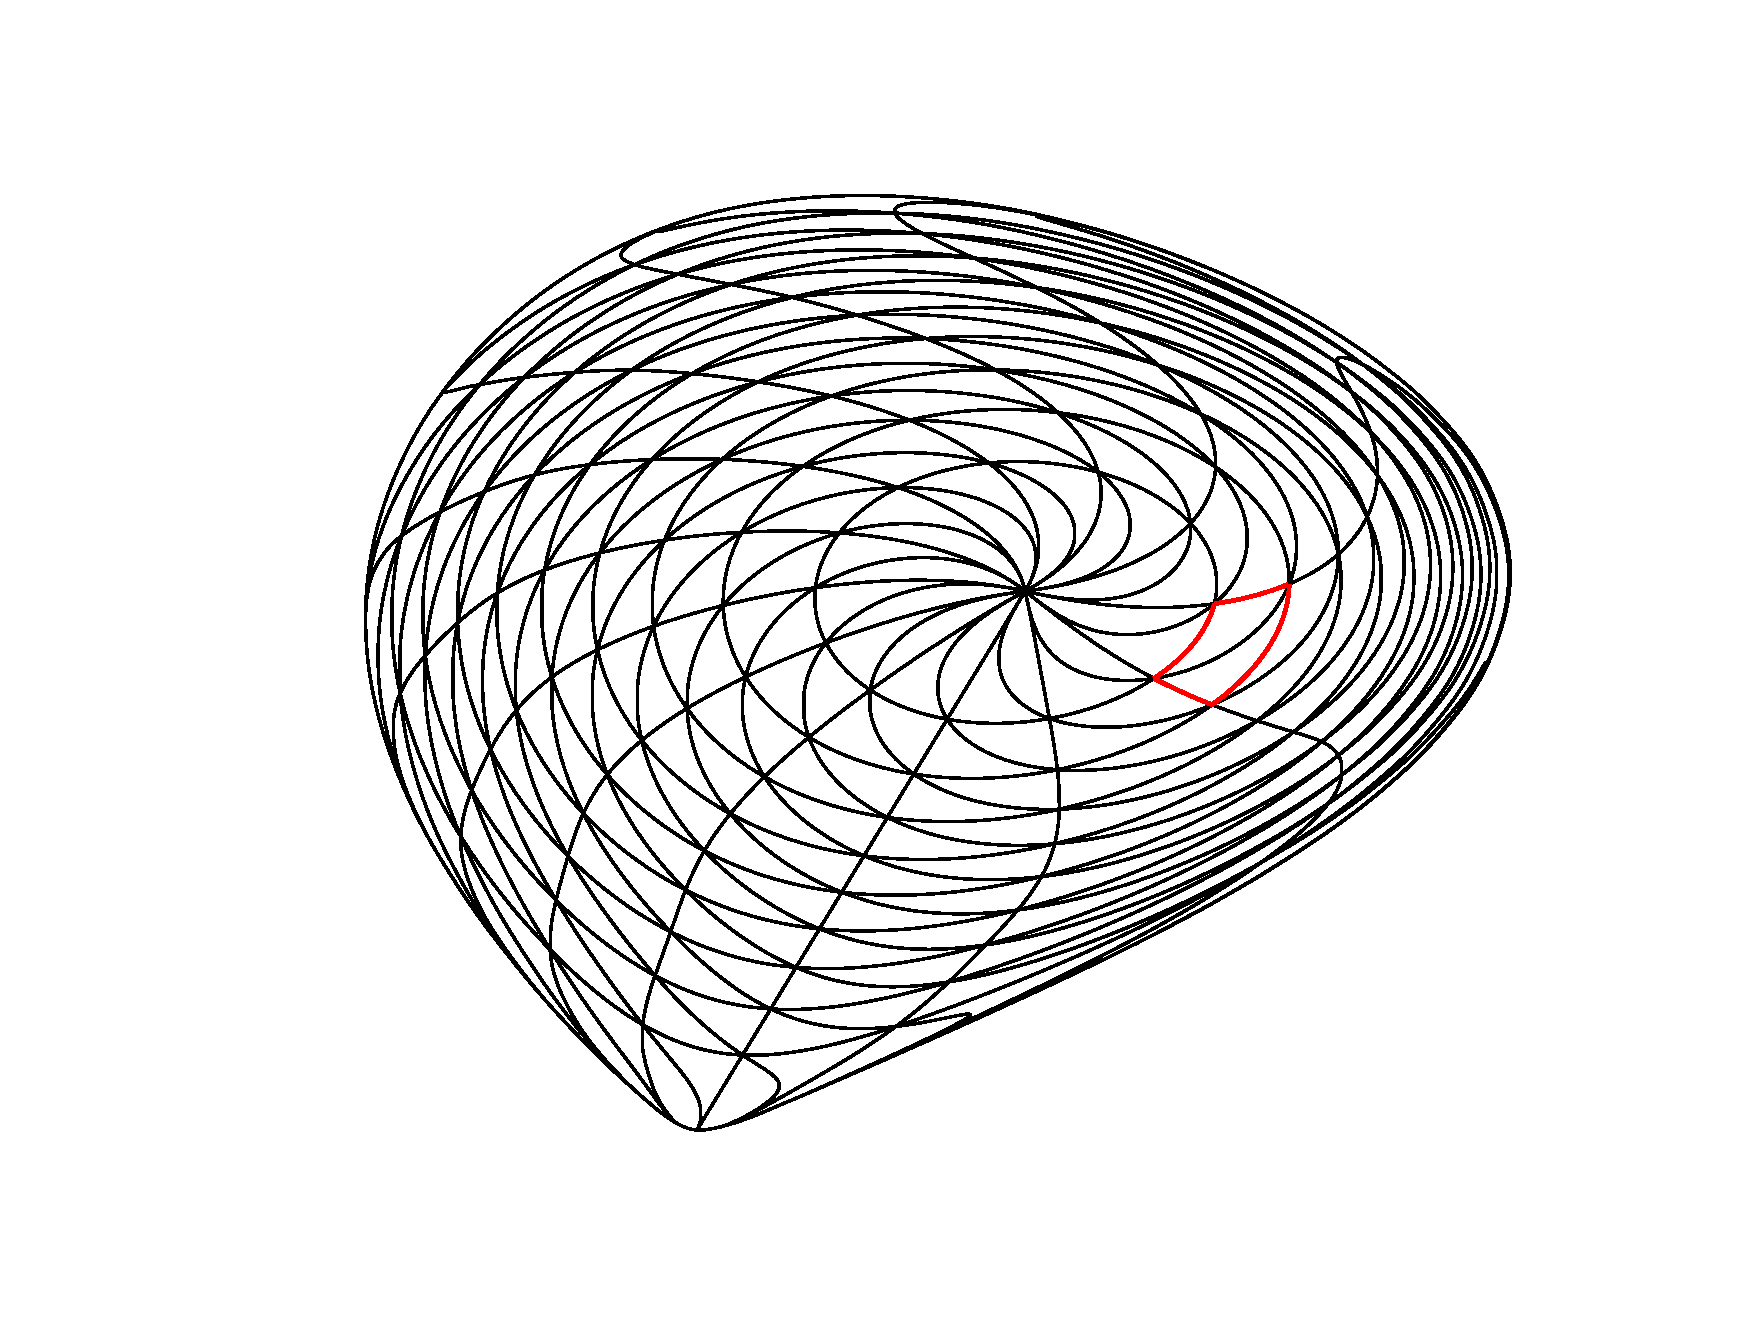
\includegraphics[width=1.0\textwidth]{figures/Curvilinear_grid.eps}
	\caption{Poloidal projection of the field aligned grid in real space, the cross sectional countour of the two combined prisms from figure \ref{fig:Curvilinear_grid_and_tetrahedra} is marked in red}
	\label{fig:Curvilinear_grid}
\end{figure}
\begin{figure}[!ht]
	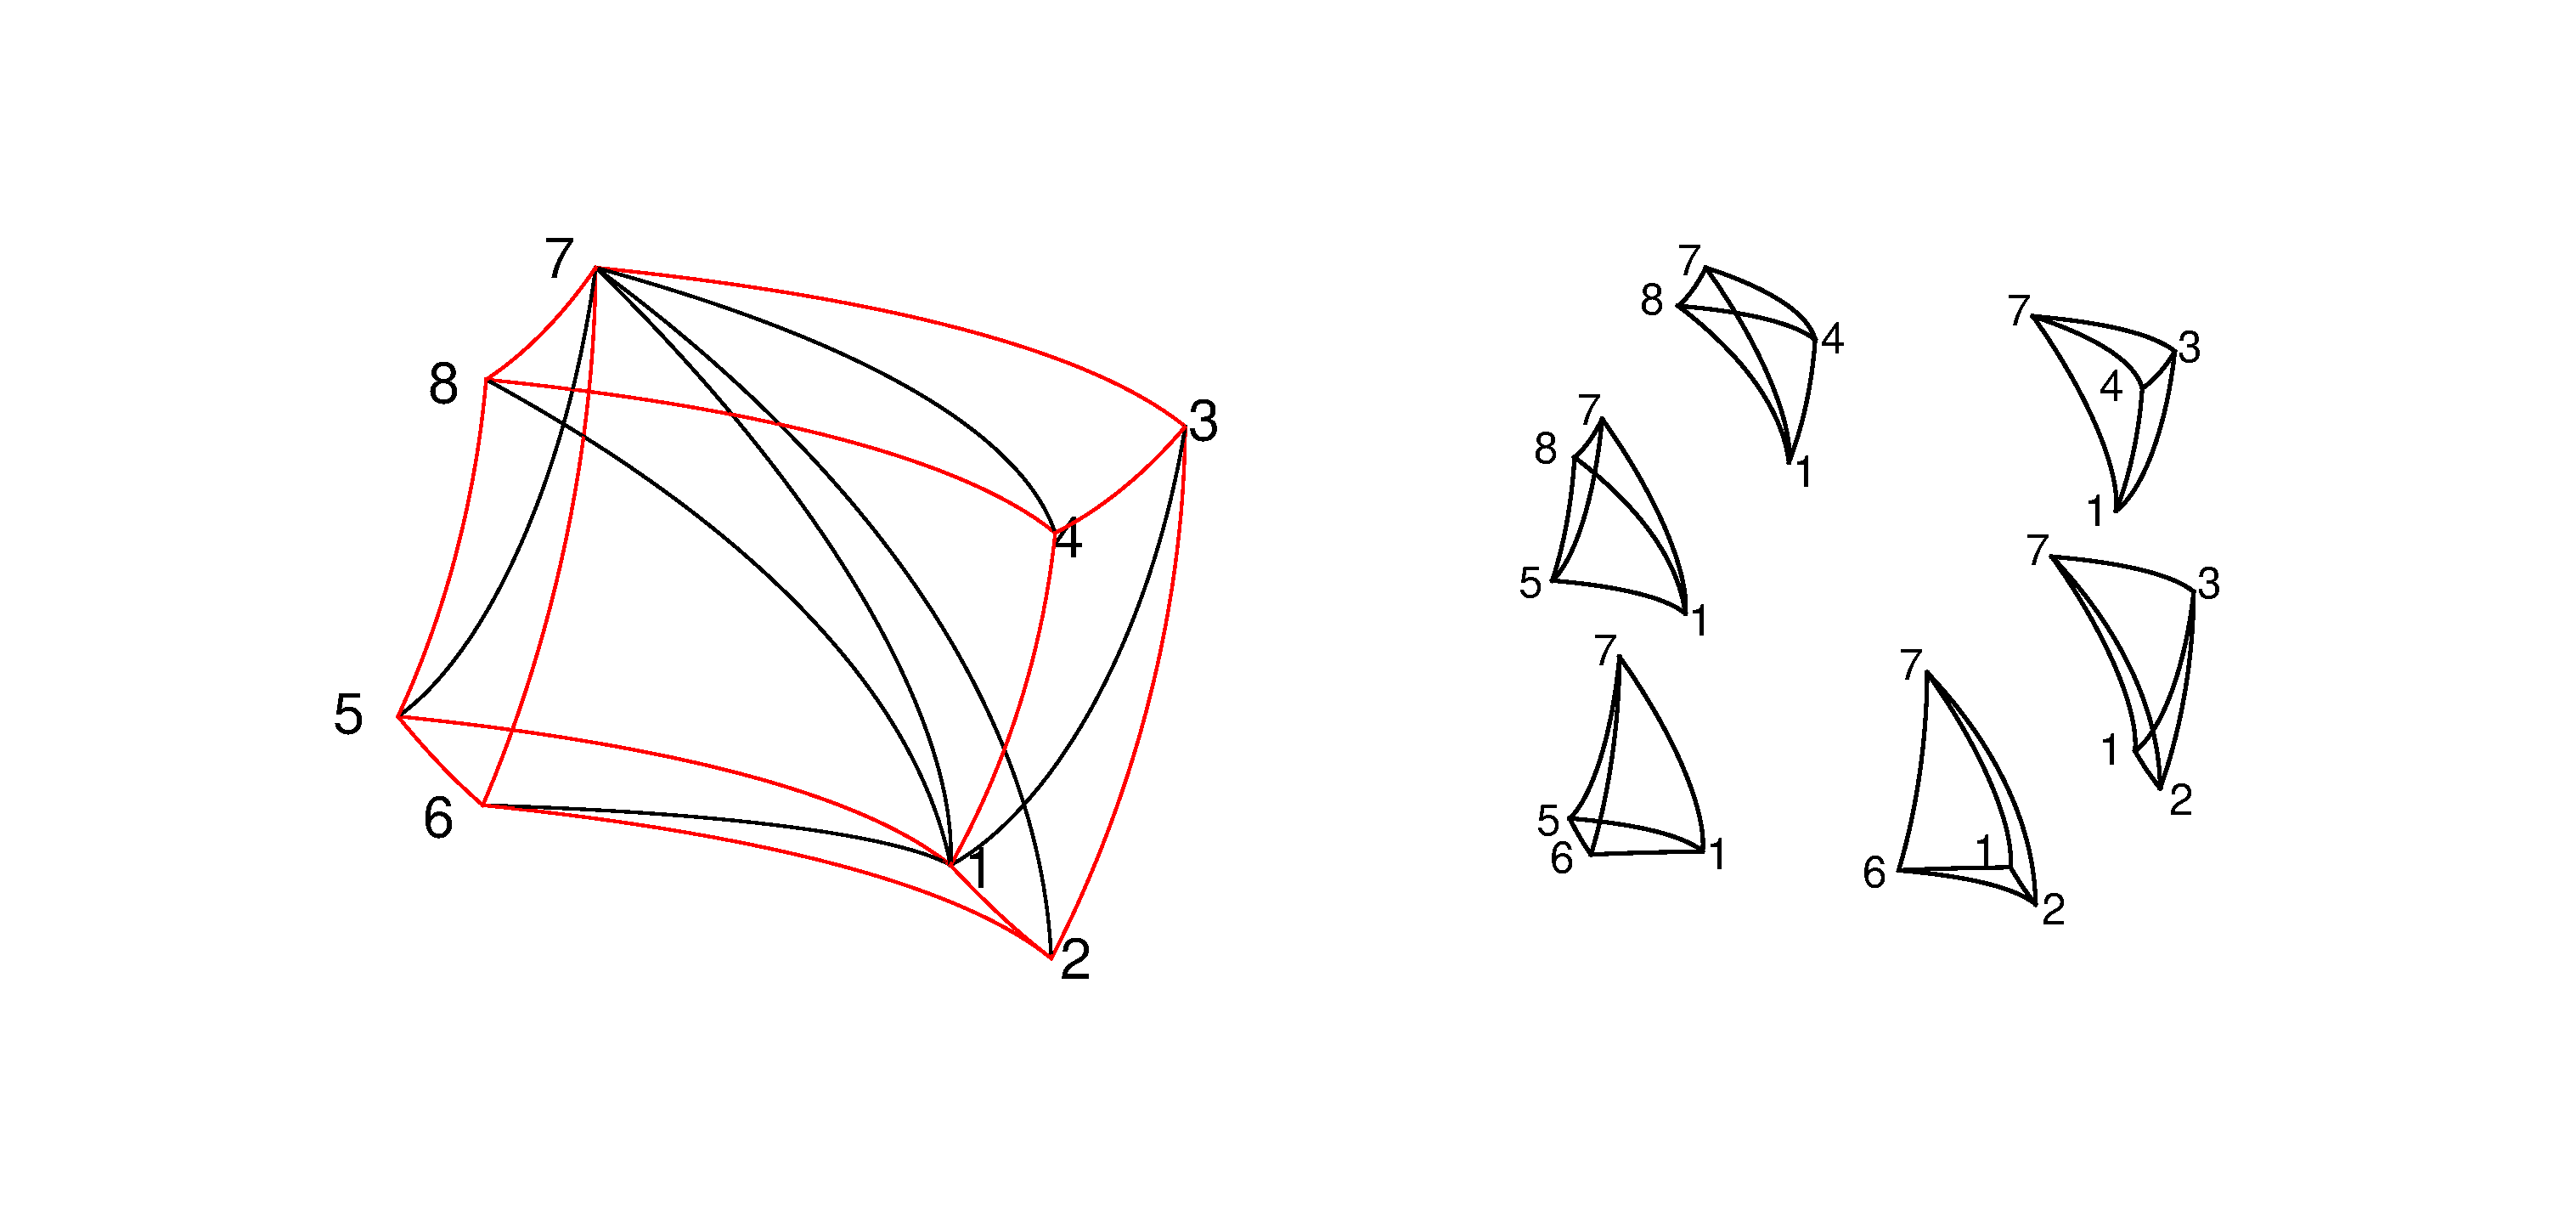
\includegraphics[width=1.0\textwidth]{figures/Curvilinear_grid_prisms_tetra.eps}
	\caption{On the left, two adjacent prisms of opposing orientation are drawn in real space with the red lines indicating how the two prisms form a hexagonal shape for a constant number of points per $\vartheta$-ring, the individual tetrahedra are plotted on the right, the corners are hereby merely indexed to enable a clearer association of the tetrahedra}
	\label{fig:Curvilinear_grid_and_tetrahedra}
\end{figure}


\end{document}